 %\documentclass[preprint,12pt]{elsarticle}

%% Use the options 1p,twocolumn; 3p; 3p,twocolumn; 5p; or 5p,twocolumn
%% for a journal layout:
%%  \documentclass[final,1p,times]{elsarticle}
%% \documentclass[final,1p,times,twocolumn]{elsarticle}
%% \documentclass[final,3p,times]{elsarticle}
%% \documentclass[final,3p,times,twocolumn]{elsarticle}
%\documentclass[final,5p,times]{elsarticle}
\documentclass[final,5p,times,twocolumn]{elsarticle}

\newcommand{\note}[2][inline]{\todo[color=red!30,#1]{\small\sf #2}}

%% if you use PostScript figures in your article
%% use the graphics package for simple commands
%% \usepackage{graphics}
%% or use the graphicx package for more complicated commands
%% \usepackage{graphicx}
%% or use the epsfig package if you prefer to use the old commands
%% \usepackage{epsfig}

%% The amssymb package provides various useful mathematical symbols
\usepackage{rotating,todonotes, xspace}
\usepackage{amssymb}
\usepackage[section]{placeins}
\usepackage{makeidx}  % allows for indexgeneration
\usepackage{algorithm}
\usepackage{algpseudocode}
\usepackage{graphicx}
\usepackage{float}
\usepackage{subcaption}
\captionsetup{compatibility=false}
\usepackage{wrapfig}
\usepackage{array}
\usepackage{multicol}
\usepackage{hyperref}
\usepackage{enumitem}

% The amsthm package provides extended theorem environments
%% \usepackage{amsthm}


\journal{Future Generation of Computer Systems}

\begin{document}

\begin{frontmatter}

%Should change the tilte to something better
\title{Using Imbalance Metrics to Optimize Task Clustering in Scientific Workflow Executions}


\author[isi]{Weiwei Chen\corref{cor1}}
\ead{weiweich@acm.org}

\author[isi]{Rafael Ferreira da Silva}
\ead{rafsilva@isi.edu}

\author[isi]{Ewa Deelman}
\ead{deelman@isi.edu}

\author[man]{Rizos Sakellariou}
\ead{rizos@cs.man.ac.uk}

\cortext[cor1]{Corresponding address: USC Information Sciences Institute, 4676 Admiralty Way Ste 1001, Marina del Rey, CA, USA, 90292, Tel: +1 310 448-8408}


\address[isi]{University of Southern California, Information Sciences Institute, Marina del Rey, CA, USA}
\address[man]{University of Manchester, School of Computer Science, Manchester, U.K.}


\begin{abstract}
Scientific workflows can be composed of many fine computational granularity tasks. The runtime of these tasks may be shorter than the duration of system overheads, for example, when using multiple resources of a cloud infrastructure. Task clustering is a runtime optimization technique that merges multiple short running tasks into a single job such that the scheduling overhead is reduced and the overall runtime performance is improved. However, existing task clustering strategies only provide a coarse-grained approach that relies on an over-simplified workflow model. In this work, we examine the reasons that cause Runtime Imbalance and Dependency Imbalance in task clustering. Then, we propose quantitative metrics to evaluate the severity of the two imbalance problems. Furthermore, we propose a series of task balancing methods (horizontal and vertical) to address the load balance problem when performing task clustering for 5 widely used scientific workflows. Finally, we analyze the relationship between these metric values and the performance of these task balancing methods. A trace-based simulation shows our methods can significantly improve the runtime performance of workflow applications when compared to a baseline execution. We also compare the performance of our methods with two algorithms from the literature.

\end{abstract}

\begin{keyword}
Scientific workflows \sep Performance analysis \sep Scheduling \sep Workflow simulation \sep Task clustering \sep Load balancing
\end{keyword}

\end{frontmatter}


\section{Introduction}
\label{intro}

Scientific workflows have been widely used on several science disciplines to manage the execution of large-scale computations~\cite{Deelman2002,Sakellariou2010,Lathers2006,Oinn2004,Wieczorek2005,Maechling2007}. 
%They consist of many computational tasks with complex data dependencies between them. 
As scientific workflows grow in complexity and importance, the research community need a deeper and broader understanding of the characteristics, features, and behaviors of workflows to drive improvements on research areas such as resource provisioning, task scheduling, and data management. 
Workflow characterization has been broadly studied by the community~\cite{Juve2013, Calasanz2008, Tolosana2011, Callaghan2011, Gunter2011, Yildiz2009, Ramakrishnan2008, Bharathi2008, Gu2013}. For instance, 
%Many computational scientists develop and use complex, data-intensive simulations and analyses~\cite{Hey2009} that are often structured as scientific workflows, which consist of many computational tasks with complex data dependencies between them. Scientific workflows continue to gain their popularity among many science disciplines, including physics~\cite{Deelman2002}, astronomy~\cite{Sakellariou2010}, biology~\cite{Lathers2006, Oinn2004}, chemistry~\cite{Wieczorek2005}, and earthquake science~\cite{Maechling2007}. 
%Researchs~\cite{Juve2013, Calasanz2008, Tolosana2011, Callaghan2011, Gunter2011, Yildiz2009, Ramakrishnan2008, Bharathi2008, Gu2013} have been conducted to elaborate the characterization of a wide variety of scientific workflows. In characterizing the execution profile for each workflow, 
Juve et al.~\cite{Juve2013} and Callaghan et al.~\cite{Callaghan2011} recently presented metrics to characterize the execution profile for each workflow as the number of job types, and I/O, memory, and CPU requirements of each type from diverse application domains. Tolosana et al.~\cite{Tolosana2011} proposed 18 metrics to characterize workflow resilience from the perspectives of the user, workflow enactor, and resource manager. Gunter et al.~\cite{Gunter2011} capture application-level logs and resource information, normalize these to standard representations, and store them in a centralized general purpose schema.

However, there are still challenges that have not been addressed yet. First, many of these workflow analysis tools use non-quantitative tools, i.e. they are neither numerical~\cite{Yildiz2009,Garijo2013} nor comparable across different platforms and workflows~\cite{Juve2013,Callaghan2011}.
%By quantitative, we first mean the metrics are numerical. Yildiz~\cite{Yildiz2009} discussed the appropriateness of standard modeling notations to scientific workflow modeling and present the basic scientific workflow structures. Garijo~\cite{Garijo2013} further introduced detection of common scientific workflow fragments using templates and execution provenance. However, these workflow structures themselves cannot serve as a criterion to evaluate the specific performance of a workflow since they are not numerical. Second, we mean these metrics must be comparable across different platforms and workflows. For example, the average task runtime~\cite{Juve2013} and the average task failure rate~\cite{Callaghan2011} are highly related to the characteristics of execution platforms (system load and resource availability etc.) and thus they do not serve as a reliable metric to guide the design of new optimization methods or a new workflow management system. 
Second, there is a lack of using structural information in these tools. Scientific workflows are typically a graph constructed by data dependencies between computational tasks.  A data dependency means there is a data transfer between two tasks (output data for one and input data for the other). Data dependencies between workflow tasks play an important role particularly with the emergence of data intensive workflows~\cite{Callaghan2011}. Existing metrics~\cite{Juve2013, Callaghan2011, Bharathi2008}  (average failure rate, average task runtime, and average resource requirement etc. ) treat workflows as no difference to workloads that have no data dependencies between them. Tolosana~\cite{Tolosana2011} has touched some basic structural information such as the average number of joins in a workflow. But such metrics cannot tell us a global picture of workflow graph such as whether this workflow is dense or sparse, whether this workflow is more sensitive to one particular part of it and whether this workflow is relatively parallel or sequential. 

Furthermore, most of these metrics ignore or underestimate the influence of system overheads that play a significant role in the workflow's runtime~\cite{Chen2011, Prodan2008, Ostberg2011}. In heterogeneous distributed systems, workflows may experience different types of overheads, which are defined as the time of performing miscellaneous work other than executing users’ computational activities. Since the causes of overheads differ, the overheads have diverse distributions and behaviors. For example, the time to run a post-script that checks the return status of a computation is usually a constant. However, queue delays incurred while tasks are waiting in a batch scheduling systems can vary widely. In our work, we add overhead as a constitution of the extended workflow graph and this approach allows to apply graph manipulations and graph-theoretic algorithms to the corresponding workflow graphs. 

Finally, the community has lacked a deep understanding of these data and how they are related to the overall performance improvement of workflows. In this paper, we propose a series of quantitative and structural metrics that are able to reflect the structure of workflow graphs. Generally speaking, we believe such metrics can (i) guide the formulation of a workflow from the perspective of designers and (ii) help workflow management systems (WMS) refine their orchestration for workflow execution (task clustering and task scheduling etc.). Specifically, in this paper we analyze three usage scenarios including workflow profiling, task clustering, and task scheduling that our metrics can be applied to as discussed below. The reason why we choose these representative areas is related to general picture of how we address issues of performance optimization in scientific workflows. 
The most straightforward approach is to invest in hardware upgrade and reduce runtime, I/O latency or network latency; for example, replacing current virtual instances with ones that have more CPU, memory or storage resources \cite{Berriman2010, Juve2012}. However, this approach results in higher IT expenses. Another solution includes varied makespan-centric, DAG scheduling algorithms and heuristics \cite{Cao2008, Dong2010, Braun2001} that have been proposed and analyzed. However, these algorithms narrow themselves to the runtime of computational or data transfer jobs. While scheduling remains an NP-hard problem, structural and overhead aware solutions can give new insight to solutions that have not been previously considered. Task clustering \cite{Chen-balanced-2013, Ferreira-granularity-2013}, job throttling \cite{Humphrey2008}, pre-staging \cite{Amer2012} and many other solutions have been proposed to reduce the impact of overheads without requiring runtime improvement of computational jobs. In this paper, we not only focus on profiling major overheads occurring in the workflow management systems and revealing their structural connections, but also propose optimization oriented metrics to improve the performance of task scheduling and task clustering. 

\textbf{Workflow Profiling} is an effective dynamic analysis approach to investigate complex applications in practice. The realistic characteristics of data-intensive workflows are critical to optimal workflow orchestration and profiling is an effective approach to investigate the behaviors of such complex applications. Traditionally, the common and straightforward approach to address issues of performance optimization is using makespan-centric, DAG scheduling algorithms~\cite{Caniou2011}. While scheduling remains an NP-hard problem, overhead analysis tools can take an important role in giving new insight to solutions that have not been previously considered and that can be further understood. Task clustering~\cite{Chen2012}, job throttling~\cite{Humphrey2008}, pre-staging~\cite{Amer2012} and many other solutions have been proposed to reduce the impact of overheads through overlapping overheads and runtimes without requiring runtime improvement of computational jobs. Instead of giving the average task runtime, in Section~\ref{sec:profiling}, we propose four metrics to reflect the projection of cumulative overheads on timeline and show how they are related to the overall performance of different workflow optimization methods.    
%The reason why we are particularly interested in reflecting the projection of overlapped overheads and runtimes is that 
%During execution on several resources, the execution time and overheads occur at the same time during execution—we name that time as overlap. We indicate how the reduction and overlap help optimize the performance. Much research is underway to address issues of performance optimization. A common and straightforward approach includes makespan-centric, DAG scheduling algorithms~\cite{Caniou2011} and heuristics that have been proposed and analyzed. However, these algorithms narrow themselves to the runtime of computational or data transfer jobs. 


\textbf{Task clustering} techniques~\cite{Ostberg2011, Chen2012, Maheshwari2012, Ferreira-granularity-2013} have been developed to group fine-grained tasks into coarse-grained tasks so that the number of computational activities is reduced and their computational granularity is increased thereby reducing the system overheads. Grouping tasks without considering these dependencies may lead to data locality problems where output data produced by parent tasks are poorly distributed~\cite{Chen-balanced-2013}. Particularly, there is a tradeoff between runtime and data dependency balancing and thus a quantitative measurement of workflow characteristics is required to serve as a criterion to select and balance these solutions. To achieve this goal, in Session~\ref{sec:imbalance}, we propose a series of metrics based on the concept of impact factor and dependency distance that reflect the internal structure (in terms of both runtime and dependency) of the workflow  and use these metrics to guide the task clustering during the runtime. 

\textbf{Task scheduling}~\cite{Caniou2011, Blythe2005, Casanova2000} has long ignored or underestimate the influence of system overheads. When executing these applications on a multi-machine distributed environment, such as the Grid or the Cloud, significant system overheads may exist~\cite{Chen2011, Prodan2008, Dong2010, Yang03, Chen2012b} and the problem of choosing robust schedules becomes more and more important. Traditionally, a carefully crafted schedule is based on deterministic or statistic estimates for the execution time of computational activities that compose a workflow. However, in such an environment, this approach may prove to be grossly inefficient~\cite{Chen2012b}, as a result of various unpredictable overheads that may occur at runtime. Thus, to mitigate the impact of uncertain overheads, it is necessary to choose a schedule that guarantees overhead robustness, that is, a schedule that is affected as little as possible by various overhead changes. In Session~\ref{sec:sensitivity}, we propose a series of structural metrics to evaluate the sensitivity of workflow performance over the overheads and further use them to guide the selection of different scheduling heuristics. 

%given a task t from a workflow w, this metric measures the relationship between the number of failures of task t and the overall number of attempts made at executing t. This could be obtained from previous executions and would provide an indicator of the frequency of failure. However, in case of abstract workflows that have their tasks mapped to resources at runtime, the frequency of failure from past executions may not accurately reflect the expected behaviour in future executions, as the reliability of resources may change during each enactment.


%Task-level QoR metrics are not appropriate for such a computation (as the number of tasks in a workflow can be high, leading to inaccurate outcomes from the statistical analysis), and the selection must be undertaken using workflow-level QoRE and/or QoRR metrics. 


%from the ParaTrac paper
% With the advance of high performance distributed computing, users are able to execute various data-intensive applications by harnessing massive computing resources [1]. Though workflow management systems have been developed to alleviate the difficulties of planning, scheduling, and executing complex workflows in distributed environments [2–5], optimal workflow management still remains a challenge because of the complexity of applications. Therefore, one of important and practical demands is to understand and characterize the data-intensive applications to help workflow management systems (WMS) refine their orchestration for workflow execution. Research has been conducted to elaborate the characterization of a wide variety of scientific workflows using synthetic approaches [6,7]. 


Together, we provide a broader overview of workflow characteristics along with the structural, quantitative and overhead aware metrics. These characterizations can be widely used by the research community to develop synthetic workflows, benchmarks, and simulations for evaluating workflow management systems. 

%The significance of this work is twofold. First, ParaTrac provides an effortless way to extract and generate informative and comprehensive workflow profiles from fine- grained profiling data, which enables users to intuitively and quantitatively analysis, debug, and refine their own workflows. Second, fine-grained profiling implies its potential support for fine-grained and realistic scheduling of workflows. Therefore, fine-grained profiling by ParaTrac suggests not only the vantage of more accurate study of workflows, but also the feasilbility of enabling more flexible workflow controls for future workflow management systems.


%Workflow analysis aims at identifying potential improvements for workflow applications by implementing analysis concerns for monitoring, measuring and controlling the behavior of workflow applications and the data used by its activities. 

%To the best of our knowledge, these problems are not tackled in unison by any existing analysis approach. To cope with these problems we propose to 

%From Gil
%2. Workflow/experiment understandability, by grouping several specific workflow templates or executions within a single abstract workflow fragment, which describes them in a more generic way. This is useful for scientists to find out the different ways of performing an abstract method.

%Good for abstract
%Design patterns have been used successfully in software development and commercial business workflows. However, in the context of scientific workflows, pattern research has not been attempted and the development of scientific workflow is based mainly on the ad-hoc copy and paste approach using previously developed workflows. Development of scientific workflow patterns will provide a formal methodology to build scientific workflow by reusing patterns that have precise semantics. Currently there is a lack of commonly agreed methodology for proposing patterns in general. Scientific workflow patterns are even harder to develop due to the data-flow oriented nature of its computation model. The simplicity of a dataflow model facilitates intuitive workflow design, analysis and optimization, however it also embeds many types of implicit dependencies such as tokens, and to- ken rate which are not present in business workflows. This increases the number of possible design patterns in contrast to business workflow that considers only activation dependencies. In this paper, we have proposed an initial set of patterns for scientific workflow models that permit data and control flow modeling. We also tested these patterns on Kepler workflow management system.

The next Section gives an overview of the related work, Section~\ref{sec:model} presents our workflow and execution environment models, Section~\ref{sec:heuristics} details our heuristics and algorithms, Section~\ref{sec:experiments} reports experiments and results, and the paper closes with a discussion and conclusions.

\section{Related Work}
\label{related}

%Workflow Profiling 
%Stampede is a workflow data model for representing the performance characteristics of distributed workflows. It can track workflow restructuring employed by workflow systems at runtime. This allows queries that reference the workflow originally defined by the user to be answered using data collected during execution. 

Some work in the literature has attempted to define and model robustness with metrics. In~\cite{Ali2004}, the authors propose a general method to define a metric for robustness. First, a performance metric is chosen. In our case, this performance metric is the overall runtime including overhead duration as we want the execution time of an application to be as stable as possible. Second, one has to identify the parameters that make the performance metric uncertain. In our case, it is the duration of the individual overheads. Third, one needs to find how a modification of these parameters changes the value of the performance metric. In our case, the answer is, as an increase of the overhead generally implies an increase of the overall runtime. 
%Lastly, one has to identify the smallest variation of a parameter that makes the performance metric exceed an acceptable bound. 
A schedule $A$ is said to be more robust than another schedule $B$ if the variation for $A$ is larger than that for $B$.
%However, estimating this variation is the most difficult part as it requires to analyze deeply the structure of the problem and its inputs.
Following this approach, Canon~\cite{Canon2008} analyzed the robustness of 20 static DAG scheduling heuristics using a metric for robustness the standard deviation of the makespan over a large number of measurement. Braun et al. \cite{Braun2001} evaluated 11 heuristics examined and for the cases studied there, the relatively simple Min-min heuristic performs well in comparison to the other techniques. 
%In comparison, we focus on varying the parameters related to overhead instead of computational tasks. 

A plethora of studies on task scheduling~\cite{Chetto1990, Dong2010, Yang03, Blythe2005} have been developed in the distributed and parallel computing domains. Many of these schedulers have been extended to consider both the computational cost and communication cost. A static or statistic estimation of communication cost or data transfer delay~\cite{Dong2010, Yang03} has been considered in the scheduling problem. In contrast, we focus on the scheduling overheads that have been ignored or underestimated for long and we demonstrate how their unique timeline patterns influence the overhead robustness. 

Workflow patterns~\cite{Yu2005, Juve2013, Liu2008} are used to capture and abstract the common structure within a workflow and they give insights on designing new workflows and optimization methods.  
Yu~\cite{Yu2005} proposed a taxonomy that characterizes and classifies various approaches for building and executing workflows on Grids. They also provided a survey of several representative Grid workflow systems developed by various projects world-wide to demonstrate the comprehensiveness of the taxonomy. Juve~\cite{Juve2013} provided a characterization of workflow from 6 scientific applications and obtained task-level performance metrics (I/O, CPU and memory consumption). They also presented an execution profile for each workflow running at a typical scale and managed by the Pegasus workflow management system~\cite{Deelman2005}. Liu~\cite{Liu2008} proposed a novel pattern based time-series forecasting strategy which ulitilizes a periodical sampling plan to build representative duration series. 
%Fix it
Compared to them, we discover a common pattern of intervals existing in system overheads while executing scientific workflows. We also leverage this knowledge to evaluate the overhead robustness of existing heuristics and develop new heuristics. 

Overhead analysis \cite{Prodan2008, Chen2011} is a topic of great interest in the grid community. Stratan \cite{Stratan2008} evaluates workflow engines including DAGMan/Condor and Karajan/Globus in a real-world grid environment. Sonmez \cite{Sonmez2006} investigated the prediction of the queue delay in grids and assessed the performance and benefit of predicting queue delays based on traces gathered from various resource and production grid environments. Prodan \cite{Prodan2008} offers a grid workflow overhead classification and a systematic measurement of overheads. Our work further investigated the major overheads and their relationship with different optimization techniques. 
In this paper, we also leverage these knowledge to enhance the existing scheduling heuristics and provide insights on designing new algorithms. 


%Many existing workflow systems provide support for capturing provenance~\cite{Gunter2011}. Profile data could be stored along with provenance to provide a more complete history of the execution of a workflow. The information could also be used to improve workflow scheduling. Many scheduling algorithms require runtime and data estimates in order to optimize workflow execution [19-22]. Profile data could be used to create a performance model of the workflow that is able to generate these estimates. Similarly, profile data could be used to guide resource provisioning algorithms that require estimates of resource usage [23-26].


%There are numerous workflow systems in use within the scientific community, for exam- ple, ASKALON [16], Kepler [3], Pegasus [12], MOTEUR [19], P-Grade [24], Taverna [28], Triana [22] and Trident [6]. Workflow standards such as the Business Process Execution Language (BPEL) [5, 29] have been applied to sci- entific problems [15]. However, there has not been much work in providing a common workflow monitoring tool 


%balancing
Task clustering~\cite{Ostberg2011, Chen2012, Maheshwari2012, Ferreira-granularity-2013} merges fined-grained tasks into coarse-grained jobs. After task clustering the number of jobs is reduced and the cumulative overhead is reduced too.
The low performance of \emph{fine-grained} tasks is a common problem in widely distributed platforms where the scheduling overhead and queuing times at resources are high, such as Grid and Cloud systems. Several works have addressed the control of task granularity of bag of tasks. For instance, Muthuvelu et al.~\cite{Muthuvelu:2005:DJG:1082290.1082297} proposed a clustering algorithm that groups bag of tasks based on their runtime---tasks are grouped up to the resource capacity. Later, they extended their work~\cite{4493929} to determine task granularity based on task file size, CPU time, and resource constraints. Recently, they proposed an online scheduling algorithm~\cite{Muthuvelu2010,Muthuvelu2013170} that groups tasks based on resource network utilization, user's budget, and application deadline. Ng et al.~\cite{keat-2006} and Ang et al.~\cite{ang-2009} introduced bandwidth in the scheduling framework to enhance the performance of task scheduling. Longer tasks are assigned to resources with better bandwidth. Liu and Liao~\cite{4958835} proposed an adaptive fine-grained job scheduling algorithm to group fine-grained tasks according to processing capacity and bandwidth of the current available resources. Although these techniques significantly reduce the impact of scheduling and queuing time overhead, they are not applicable to scientific workflows, since data dependencies are not considered.


%should fix it
%We now briefly describe the scientific workflows that we have characterized.Montage: Montage [2] was created by the NASA/IPAC Infrared Science Archive as an open source toolkit that can be used to generate custom mosaics of the sky using input images in the Flexible Image Transport System (FITS) format. During the production of the final mosaic, the geometry of the output image is calculated from the input images. The inputs are then re-projected to have the same spatial scale and rotation, the background emissions in the images are corrected to have a uniform level, and the re-projected, corrected images are co-added to form the output mosaic. The Montage application has been represented as a workflow that can be executed in Grid environments such as the TeraGrid [30].CyberShake: The CyberShake workflow [31] is used by the Southern California Earthquake Center (SCEC) [32] to characterize earthquake hazards using the Probabilistic Seismic Hazard Analysis (PSHA) technique. Given a region of interest, an MPI based finite difference simulation is performed to generate Strain Green Tensors (SGTs). From the SGT data, synthetic seismograms are calculated for each of a series of predicted ruptures. Once this is done, spectral acceleration and probabilistic hazard curves are calculated from the seismograms to characterize the seismic hazard. CyberShake workflows composed of more than 800,000 jobs have been executed using the Pegasus workflow management system on the TeraGrid [33, 34]. Broadband: Broadband is a computational platform used by the Southern California Earthquake Center [32]. The objective of Broadband is to integrate a collection of motion simulation codes and calculations to produce research results of value to earthquake engineers. These codes are composed into a workflow that simulates the impact of one or more earthquakes on one of several recording stations. Researchers can use the Broadband platform to combine low frequency (less than 1.0Hz) deterministic seismograms with high frequency (∼10Hz) stochastic seismograms and calculate various ground motion intensity measures (spectral acceleration, peak ground acceleration and peak ground velocity) for building design analysis.Epigenomics: The USC Epigenome Center [35] is currently involved in mapping the epigenetic state of human cells on a genome-wide scale. The Epigenomics workflow is essentially a data processing pipeline that uses the Pegasus workflow management system to automate the execution of the various genome sequencing operations. DNA sequence data generated by the Illumina-Solexa [36] Genetic Analyzer system is split into several chunks that can be operated on in parallel. The data in each chunk is converted into a file format that can be used by the Maq software that maps short DNA sequencing reads [37, 38]. From there, the sequences are filtered to remove noisy and contaminating segments and mapped into the correct location in a reference genome, Finally, a global map of the aligned sequences is generated and the sequence density at each position in the genome is calculated. This workflow is being used by the Epigenome Center in the processing of production DNA methylation and histone modification data.LIGO Inspiral Analysis: The Laser Interferometer Gravitational Wave Observatory (LIGO) [39, 40] is attempting to detect gravitational waves produced by various events in the universe as per Einstein’s theory of general relativity. The LIGO Inspiral Analysis workflow [41] is used to analyze the data obtained from the coalescing of compact binary systems such as binary neutron stars and black holes. The time-frequency data from each of the three LIGO detectors is split into smaller blocks for analysis. For each block, the workflow generates a subset of waveforms belonging to the parameter space and computes the matched filter output. If a true inspiral has been detected, a trigger is generated that can be checked with triggers for the other detectors. Several additional consistency tests may also be added to the workflow.SIPHT: The bioinformatics project at Harvard University is conducting a wide search for small, untranslated RNAs (sRNAs) that regulate processes such as secretion and virulence in bacteria. The sRNA Identification Protocol using High-throughput Technology (SIPHT) program [42] uses a workflow to automate the search for sRNA encoding-genes for all bacterial replicons in the National Center for Biotechnology Information (NCBI) database. The kingdom-wide prediction and annotation of sRNA encoding genes involves a variety of programs that are executed in the proper order using Condor DAGMan’s [43, 44] capabilities. These involve the prediction of Rho-independent transcriptional terminators, BLAST (Basic Local Alignment Search Tools) comparisons of the inter-genetic regions of different replicons and the annotations of any sRNAs that are found.



% Section
\section{Related Work}
\label{sec:related-work}

The low performance of \emph{fine-grained} tasks is a common problem in widely distributed platforms where the scheduling overhead and queuing times at resources are high, such as Grid and Cloud systems. Several works have addressed the control of task granularity of bag of tasks. For instance, Muthuvelu et al.~\cite{Muthuvelu:2005:DJG:1082290.1082297} proposed a clustering algorithm that groups bag of tasks based on their runtime---tasks are grouped up to the resource capacity. Later, they extended their work~\cite{4493929} to determine task granularity based on task file size, CPU time, and resource constraints. Recently, they proposed an online scheduling algorithm~\cite{Muthuvelu2010,Muthuvelu2013170} that groups tasks based on resource network utilization, user's budget, and application deadline. Ng et al.~\cite{keat-2006} and Ang et al.~\cite{ang-2009} introduced bandwidth in the scheduling framework to enhance the performance of task scheduling. Longer tasks are assigned to resources with better bandwidth. Liu and Liao~\cite{Liu2009} proposed an adaptive fine-grained job scheduling algorithm to group fine-grained tasks according to processing capacity and bandwidth of the current available resources. Although these techniques significantly reduce the impact of scheduling and queuing time overhead, they are not applicable to scientific workflows, since data dependencies are not considered.

Task granularity control has also been addressed in scientific workflows. For instance, Singh et al.~\cite{Singh:2008:WTC:1341811.1341822} proposed a level- and label-based clustering. In level-based clustering, tasks at the same level can be clustered together. The number of clusters or tasks per cluster are specified by the user. In the label-based clustering, the user labels tasks that should be clustered together. Although their work considers data dependency between workflow levels, it is done manually by the users, which is prone to errors. Recently, Ferreira da Silva et al.~\cite{Ferreira-granularity-2013} proposed task grouping and ungrouping algorithms to control workflow task granularity in a non-clairvoyant and online context, where none or few characteristics about the application or resources are known in advance. Their work significantly reduced scheduling and queuing time overheads, but did not consider data dependencies.

A plethora of balanced scheduling algorithms have been developed in the networking and operating system domains. Many of these schedulers have been extended to the hierarchical setting. Lifflander et al.~\cite{Lifflander} proposed to use work stealing and a hierarchical persistence-based rebalancing algorithm to address the imbalance problem in scheduling. Zheng et al.~\cite{Zheng} presented an automatic hierarchical load balancing method that overcomes the scalability challenges of centralized schemes and poor solutions of traditional distributed schemes. There are other scheduling algorithms~\cite{Braun2001} (e.g. list scheduling) that indirectly achieve load balancing of workflows through makespan minimization. However, the benefit that can be achieved through traditional scheduling optimization is limited by its complexity. The performance gain of task clustering is primarily determined by the ratio between system overheads and task runtime, which is more substantial in modern distributed systems such as Clouds and Grids. 
\section{Model and Design}
\label{sec:model}


A workflow is modeled as a directed acyclic graph (DAG), where each node in the DAG often represents a workflow task ($t$), and the edges represent dependencies between the tasks that constrain the order in which tasks are executed. Dependencies typically represent data-flow dependencies in the application, where the output files produced by one task are used as inputs of another task. Each task is a computational program and a set of parameters that need to be executed. Figure~\ref{fig:model_odag} (left) shows an illustration of a DAG composed of four tasks. This model fits several workflow management systems such as Pegasus~\cite{Deelman:2005:PFM:1239649.1239653}, Askalon~\cite{Fahringer:2005:ATS:1064323.1064331}, and Taverna~\cite{Oinn:2006:TLC:1148437.1148448}. In this paper, we assume there is only one execution site and there is no sub-workflow or workflow partitioning~\cite{6217508}. 

\begin{figure}[!htb]
	\centering
	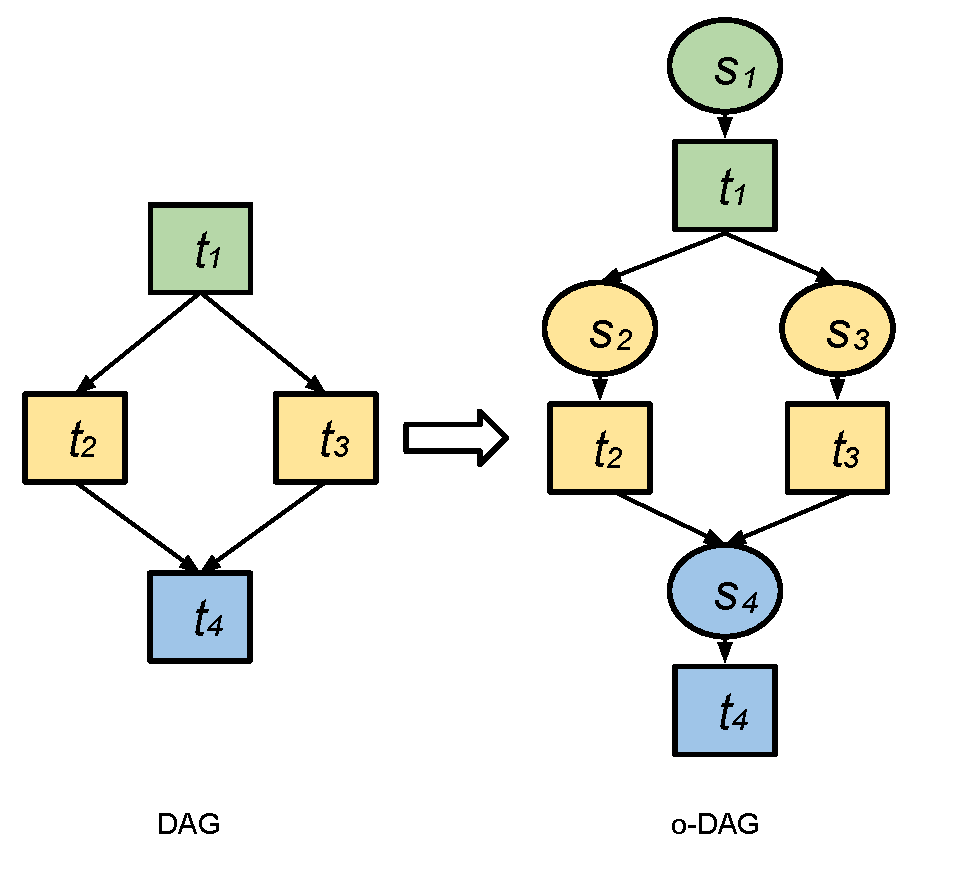
\includegraphics[width=0.7\linewidth]{figures/model/odag_color.pdf}
	\captionof{figure}{Extending DAG to o-DAG. "s" denotes a system overhead. }
	\label{fig:model_odag}
\end{figure}

Figure~\ref{fig:model_system} shows a typical workflow execution environment. The submit host prepares a workflow for execution (clustering, mapping, etc.), and worker nodes, at an execution site, execute jobs individually. The main components are introduced below:

\begin{figure}[!htb]
\centering
  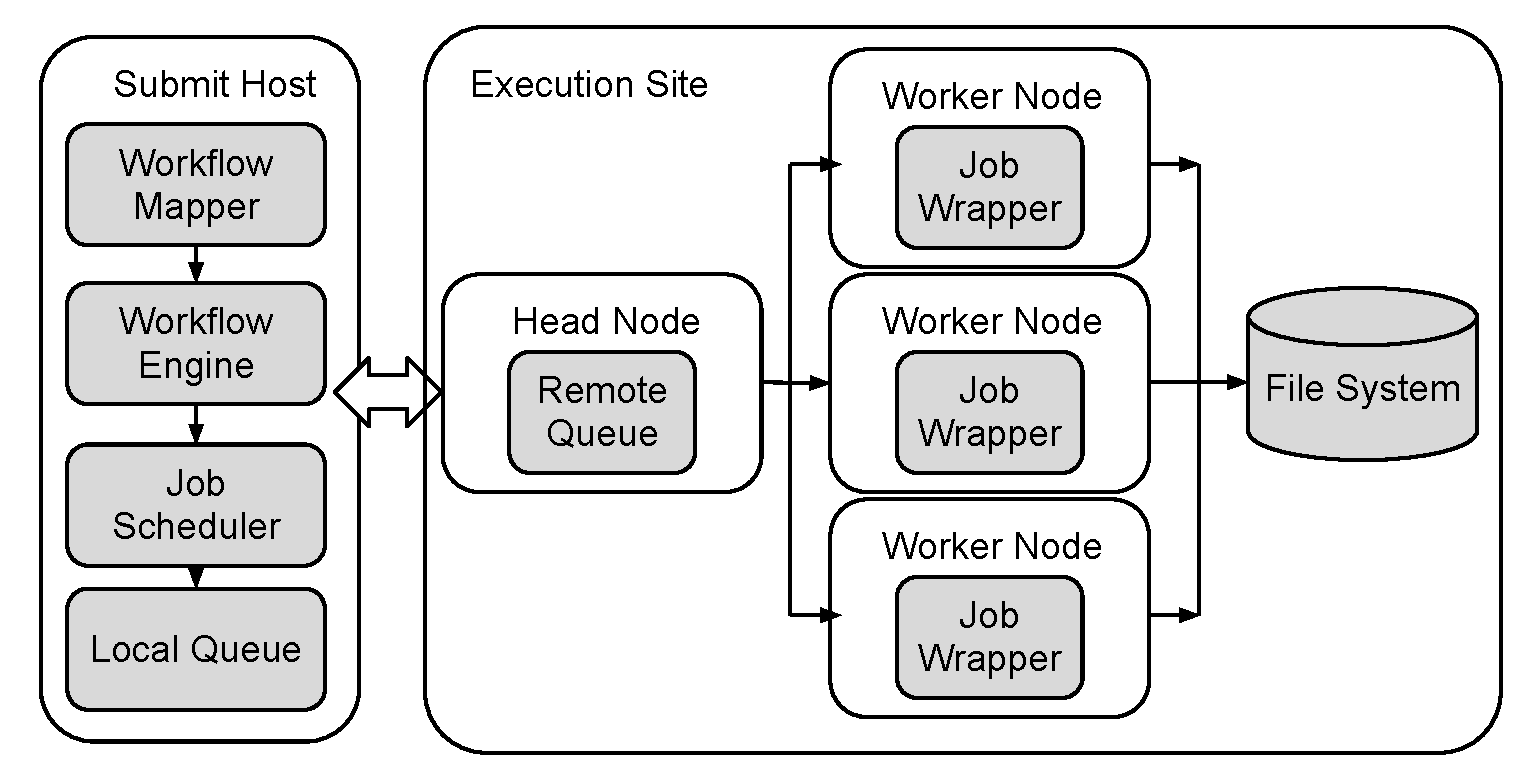
\includegraphics[width=0.95\linewidth]{figures/model/execution.pdf}
  \caption{A workflow system model.}
  \label{fig:model_system}
\end{figure}

\paragraph{Workflow Mapper} Generates an executable workflow based on an abstract workflow provided by the user or workflow composition system. It also restructures the workflow to optimize performance and adds tasks for data management and provenance information generation. In this work, the workflow mapper is used to merge small tasks together into a job such that system overheads are reduced (\textbf{task clustering}). A job is a single execution unit in the workflow execution systems and is composed of one or more tasks. 


\paragraph{Workflow Engine} Executes jobs defined by the workflow in order of their dependencies. Only jobs that have all their parent jobs completed are submitted to the Job Scheduler. The Workflow Engine relies on the resources (compute, storage, and network) defined in the executable workflow to perform computations. The elapsed time from when a job is released (all of its parents have completed successfully) to when it is submitted to the job scheduler is denoted the workflow engine delay. %The workflow engine delay is usually configured by users to assure that the entire workflow scheduling and execution system is not overloaded. 

\paragraph{Job Scheduler and Local Queue} Manage individual workflow jobs and supervise their execution on local and remote resources. The elapsed time from when a task is submitted to the job scheduler to when it starts its execution in a worker node is denoted as the queue delay. It reflects both the efficiency of the job scheduler and the resource availability. 

\paragraph{Job Wrapper} Extracts tasks from clustered jobs and executes them at the worker nodes. The clustering delay is the  elapsed time of the extraction process.

We extend the DAG model to be overhead aware (o-DAG). System overheads play an important role in workflow execution and constitute a major part of the overall runtime when tasks are poorly clustered~\cite{Chen2011}. Figure~\ref{fig:model_odag} shows how we augment a DAG to be an o-DAG with the capability to represent system overheads ($s$) such as workflow engine and queue delays. In addition, system overheads also include data transfer delay caused by staging-in and staging-out data. This classification of system overheads is based on our prior study on workflow analysis~\cite{Chen2011}. 

With an o-DAG model, we can explicitly express the process of task clustering. In this work, we address task clustering horizontally and vertically. \textbf{Horizontal Clustering} (HC) merges multiple tasks that are at the same horizontal level of the workflow, in which task horizontal level is defined as the furthest distance from the root task to this task. \textbf{Vertical Clustering} (VC) merges tasks within a pipeline of the workflow. Tasks at the same pipeline share a single-parent-single-child relationship, which means a task $t_a$ is the unique parent of a task $t_b$, which is the unique child of $t_a$. 

Figure~\ref{fig:model_hc} shows a simple example of how to perform HC, in which two tasks $t_2$ and $t_3$, without data dependency between them, are merged into a clustered job $j_1$. A job $j$ is a single execution unit composed by one or multiple task(s). Job wrappers are commonly used to execute clustered jobs, but they add an overhead denoted the clustering delay $c$. The clustering delay measures the difference between the sum of the actual task runtimes and the job runtime seen by the job scheduler. 
After horizontal clustering, $t_2$ and $t_3$ in $j_1$ can be executed in sequence or in parallel, if supported. In this work, we consider sequential executions only. Given a single resource, the overall runtime for the workflow in Figure~\ref{fig:model_hc} (left) is $runtime_l= \sum_{i=1}^{4}(s_i+t_i)$, and the overall runtime for the clustered workflow in Figure~\ref{fig:model_hc} (right) is $runtime_r=s_1+t_1+s_2+c_1+t_2+t_3+s_4+t_4$.  $runtime_l > runtime_r$ as long as $c_1 < s_3$, which is the case in many distributed systems since the clustering delay within an execution node is usually shorter than the scheduling overhead across different execution nodes. 

\begin{figure}[!htb]
\centering
 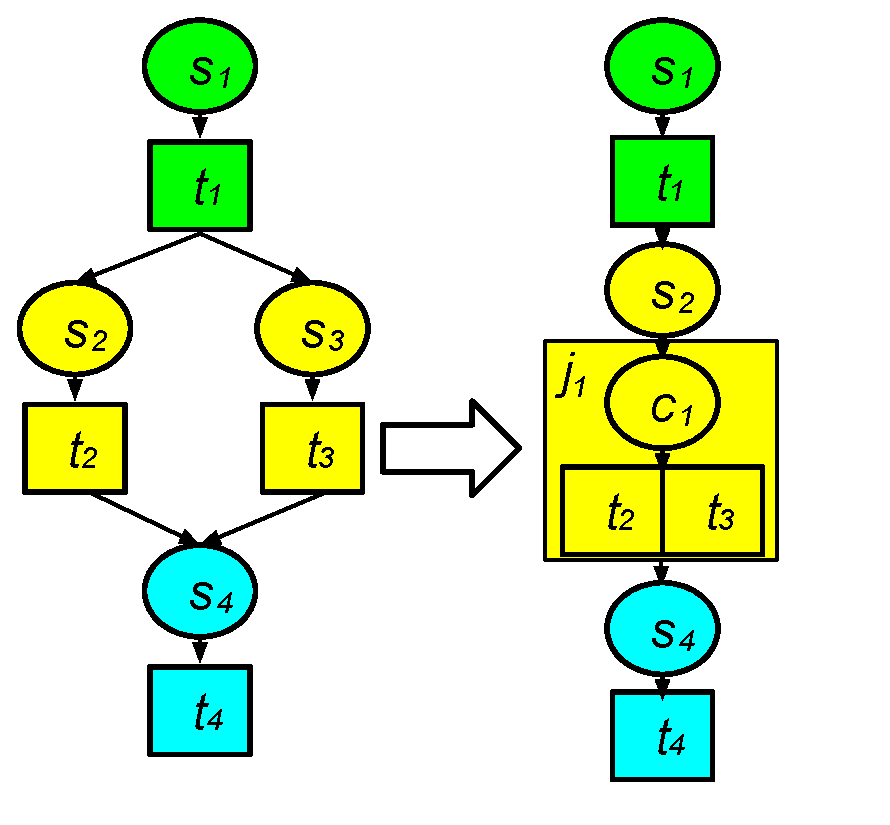
\includegraphics[width=0.55\linewidth]{figures/model/hc_color.pdf}
  \captionof{figure}{An example of horizontal clustering (color indicates the horizontal level of a task).}
  \label{fig:model_hc}
\end{figure}

Figure~\ref{fig:model_vc} illustrates an example of vertical clustering, in which tasks $t_2$, $t_4$, and $t_6$ are merged into $j_1$, while tasks $t_3$, $t_5$, and $t_7$ are merged into $j_2$. Similarly, clustering delays $c_2$ and $c_3$ are added to $j_1$ and $j_2$ respectively, but system overheads $s_4$, $s_5$, $s_6$, and $s_7$ are removed. 

\begin{figure}[!htb]
\centering
 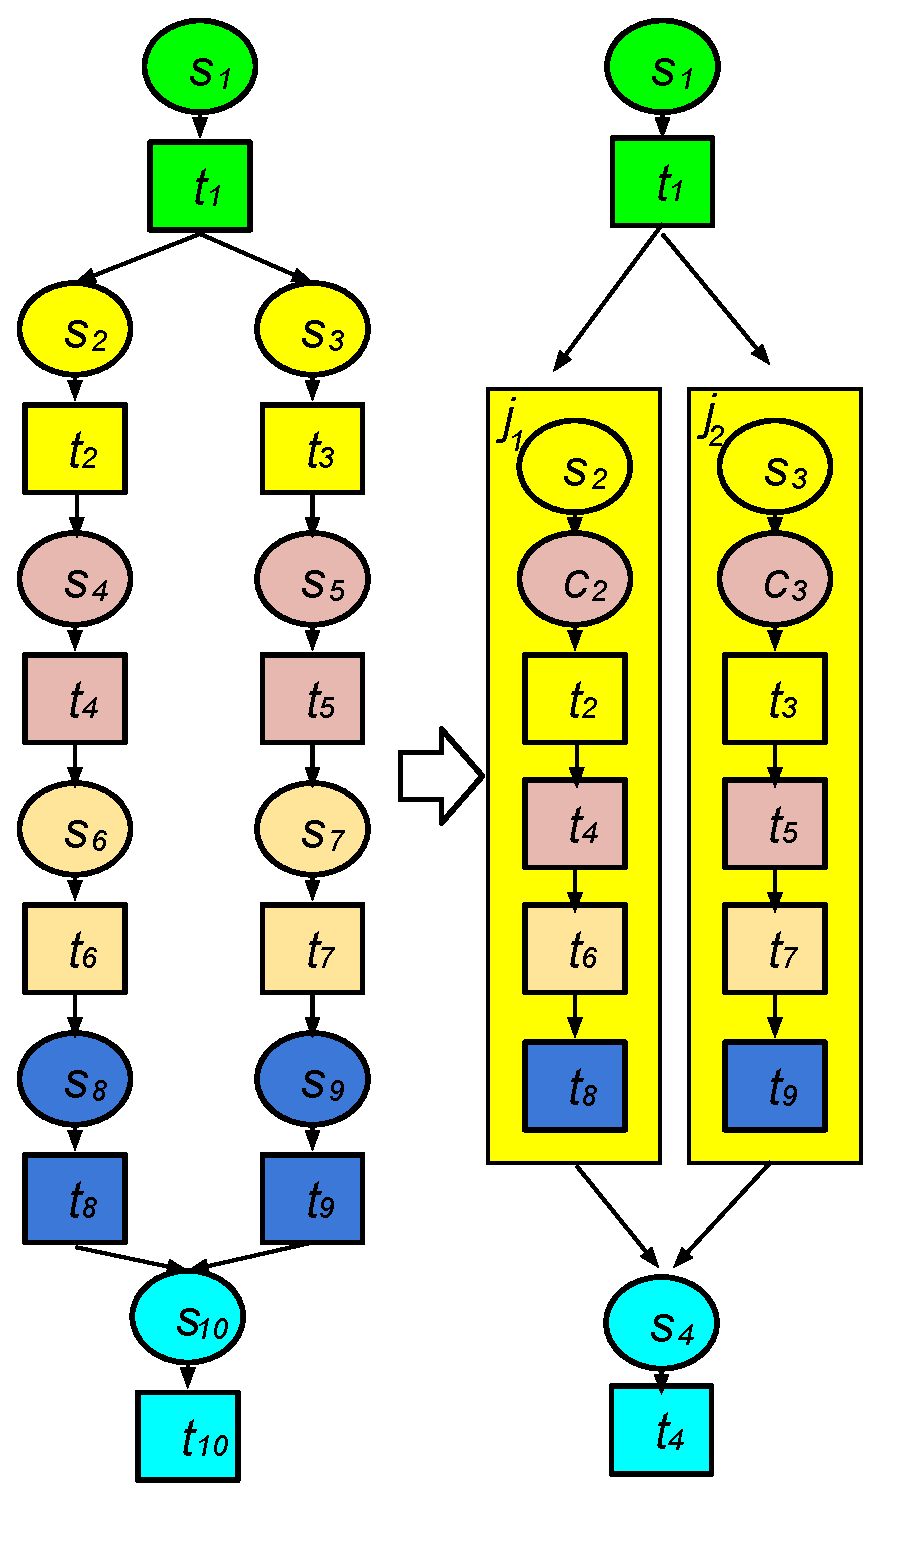
\includegraphics[width=0.6\linewidth]{figures/model/vc_color.pdf}
  \captionof{figure}{An example of vertical clustering.}
  \label{fig:model_vc}
\end{figure}

%Task clustering has been applied to many scenarios where resources are much less than tasks, which is true for many scientific workflows~\cite{Singh2008, Ying2009, Zomaya2004}, and has achieved significant improvement (i.e., 97\% as reported by ~\cite{Singh2008}) over the case without clustering. Table~\ref{tab:model_stats} shows the statistical workflow information (average task runtime etc. ) of six widely used scientific applications and their runtime information (number of nodes, average queue delay, etc.)~\cite{Chen2011}. For all of these workflows, there are a lot more tasks than available nodes and the average task runtime is shorted than system overheads. Therefore, task clustering can achieve significant improvement over no clustering. Besides the benefits of runtime improvement, task clustering also allows us to run on some federated distributed environment. For example, FutureGrid~\cite{FutureGrid} allows a user to use up to 20 VMs at a time. We will introduce the details of these workflows and distributed platforms in Session~\ref{sec:experiments}

%\begin{table*}[htbp]
%\centering
%\begin{tabular}{lrrrrrrrr}
%\hline
%Workflow & Venue & Nodes & Tasks & Workflow Engine Delay  &  Queue Delay  & Task Runtime  \\
%
%\hline
%
%SIPHT & UW Madison & 8 & 33 & 17 & 69 & 20\\ 
%Broadband & Amazon EC2 & 8 &770 & 17 &945&308\\
%Epigenomics &Amazon EC2&8& 83 &6&311&158\\
%CyberShake &Skynet&5&24142&12&188&5\\
%Montage &USC&20&10427&182&26136&523\\
%
%
%\hline
%\end{tabular}
%\caption{Overhead (in seconds) and Runtime Information }
%\label{tab:model_stats}
%\end{table*} 

\section{Balanced Clustering}
\label{sec:imbalance}

Task clustering has been widely used to address the low performance of very short running tasks on platforms where the system overhead is high, such as distributed computing infrastructures. However, up to now, techniques do not consider the load balance problem. In particular, merging tasks within a workflow level without considering the runtime variance may cause load imbalance (Runtime Imbalance), or merging tasks without considering their data dependencies may lead the system to data locality problems (Dependency Imbalance). In this section, we introduce metrics that quantitatively capture workflow characteristics to measure runtime and dependence imbalances. We then present methods to handle the load balance problem.


\subsection{Imbalance metrics}

\textbf{Runtime Imbalance} describes the difference of the task/job runtime of a group of tasks/jobs. In this work, we denote the \textbf{Horizontal Runtime Variance} ($HRV$) as the ratio of the standard deviation in task runtime to the average runtime of tasks/jobs at the same horizontal level of a workflow. At the same horizontal level, the job with the longest runtime often controls the release of the next level jobs. A high $HRV$ value means that the release of next level jobs has been delayed. Therefore, to improve runtime performance, it is meaningful to reduce the standard deviation of job runtime. Figure~\ref{fig:imbalance_rv} shows an example of four independent tasks $t_1$, $t_2$, $t_3$ and $t_4$ where the task runtime of $t_1$ and $t_2$ is 10 seconds, and the task runtime of $t_3$ and $t_4$ is 30 seconds. In the Horizontal Clustering (HC) approach, a possible clustering result could be merging $t_1$ and $t_2$ into a clustered job, and $t_3$ and $t_4$ into another. This approach results in imbalanced runtime, i.e., $HRV > 0$ (Figure~\ref{fig:imbalance_rv}-top). In contrast, a balanced clustering strategy should try its best to evenly distribute task runtime among jobs as shown in Figure~\ref{fig:imbalance_rv} (bottom). A smaller \emph{HRV} means that the runtime of tasks within a horizontal level is more evenly distributed and therefore it is less necessary to balance the runtime distribution. However, runtime variance is not able to describe how regular is the structure of the dependencies between tasks.

\begin{figure}[htb]
	\centering
	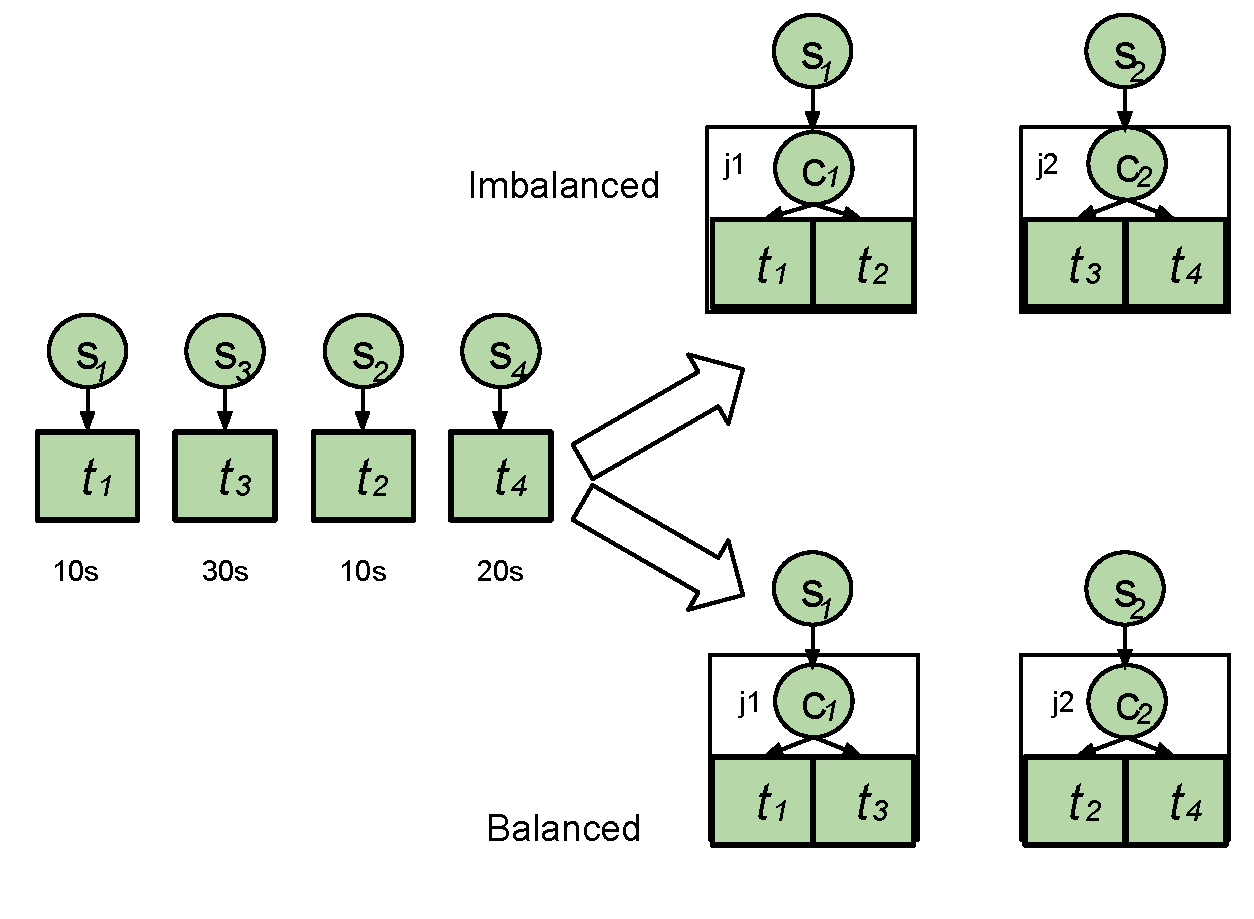
\includegraphics[width=0.95\linewidth]{figures/imbalance/runtime_variance.pdf}
	\captionof{figure}{An example of Horizontal Runtime Variance.}
	\label{fig:imbalance_rv}
\end{figure}


\textbf{Dependency Imbalance} means that the task clustering at one horizontal level forces the tasks at the next level (or even subsequent levels) to have severe data locality problems and thus loss of parallelism. For example, in Figure~\ref{fig:imbalance_dv}, we show a two-level workflow composed of four tasks in the first level and two in the second. Merging $t_1$ with $t_3$ and $t_2$ with $t_4$ (imbalanced workflow in Figure~\ref{fig:imbalance_dv}) forces $t_5$ and $t_6$ to transfer files from two locations and wait for the completion of $t_1$, $t_2$, $t_3$, and $t_4$.  A balanced clustering strategy groups tasks that have the maximum number of child tasks in common. Thus, $t_5$ can start to execute as soon as $t_1$ and $t_2$ are completed, and so can $t_6$. To measure and quantitatively demonstrate the Dependency Imbalance of a workflow, we propose two  metrics: ($i$) Impact Factor Variance, and ($ii$) Distance Variance. 

\begin{figure}[htb]
	\centering
	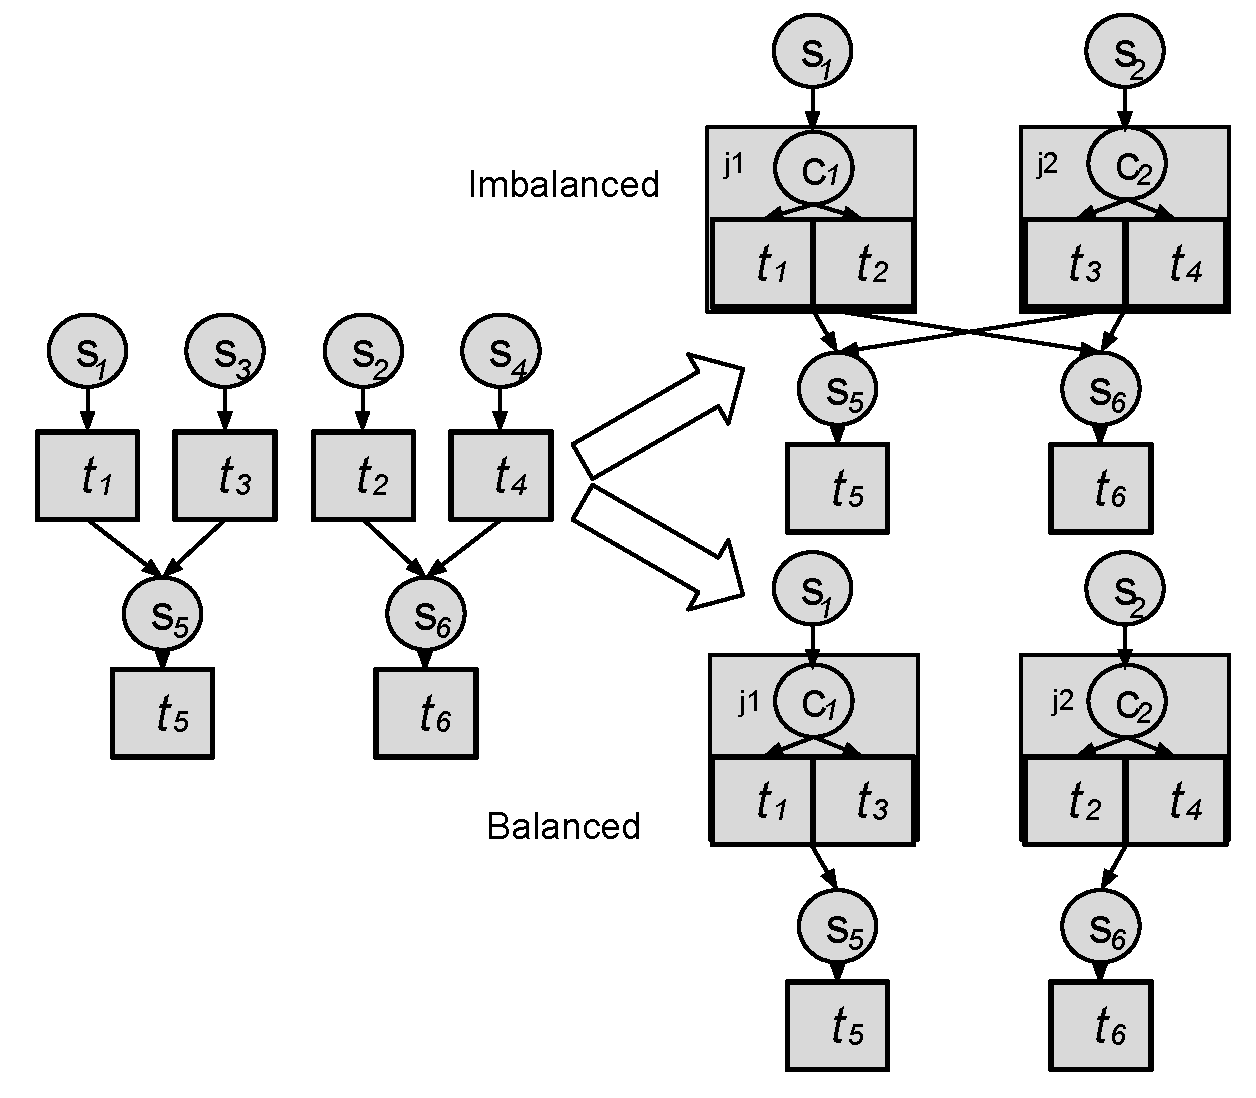
\includegraphics[width=0.95\linewidth]{figures/imbalance/dv.pdf}
	\captionof{figure}{An example of Dependency Imbalance.}
	\label{fig:imbalance_dv}
\end{figure}

We define the \textbf{Impact Factor Variance} ($IFV$) of tasks as the standard deviation of their impact factors. The Impact Factor aims at capturing the similarity of tasks/jobs in a graph by measuring their relative impact factor or importance to the entire graph. Tasks with similar impact factors are merged together, so that the workflow structure tends to be more `even' or `regular'. The \textbf{Impact Factor} ($IF$) of a task $t_u$ is defined as follows:

\begin{equation}
\label{eq:imbalance_impact_factor}
	IF(t_u)=\sum_{t_v\in Child(t_u)}^{}\frac{IF(t_v)}{||Parent(t_v)||}
\end{equation}
where $Child(t_u)$ denotes the set of child tasks of $t_u$, and $||Parent(t_v)||$ the number of parent tasks of $t_v$. For simplicity, we assume the $IF$ of a workflow exit task (e.g. $t_5$ in Figure~\ref{fig:imbalance_dv}) as 1.0. For instance, consider the two workflows presented in Figure~\ref{fig:imbalance_hifv}. $IF$ for $t_1$, $t_2$, $t_3$, and $t_4$ are computed as follows:

\begin{eqnarray}
	\displaystyle  
	&IF(t_7 )=1.0, IF(t_6 )=IF(t_5 )=IF(t_7 )/2=0.5\nonumber  \\
	&IF(t_1 )=IF(t_2 )=IF(t_5 )/2=0.25\nonumber \\
	&IF(t_3 )=IF(t_4 )=IF(t_6 )/2=0.25\nonumber 
\end{eqnarray}
Thus, IFV($t_1$, $t_2$, $t_3$, $t_4$) = 0. In contrast, $IF$ for $t_{1'}$, $t_{2'}$, $t_{3'}$, and $t_{4'}$ are:

\begin{eqnarray}
	\displaystyle  
	&IF(t_{7'})=1.0, IF(t_{6'})=IF(t_{5'})=IF(t_{1'})=IF(t_{7'})/2=0.5\nonumber \\
	&IF(t_{2'})=IF(t_{3'})=IF(t_{4'})=IF(t_{6'})/3=0.17 \nonumber
\end{eqnarray}
Therefore, the $IFV$ value for {$t_{1'}$, $t_{2'}$, $t_{3'}$, $t_{4'}$} is 0.17, which means it is less regular than the workflow in Figure~\ref{fig:imbalance_hifv} (left). In this work, we use \textbf{HIFV} (Horizontal IFV) to indicate the $IFV$ of tasks at the same horizontal level. The time complexity of calculating all the $IF$ of a workflow with $n$ tasks is $O(n)$.  

\begin{figure}[htb]
	\centering
	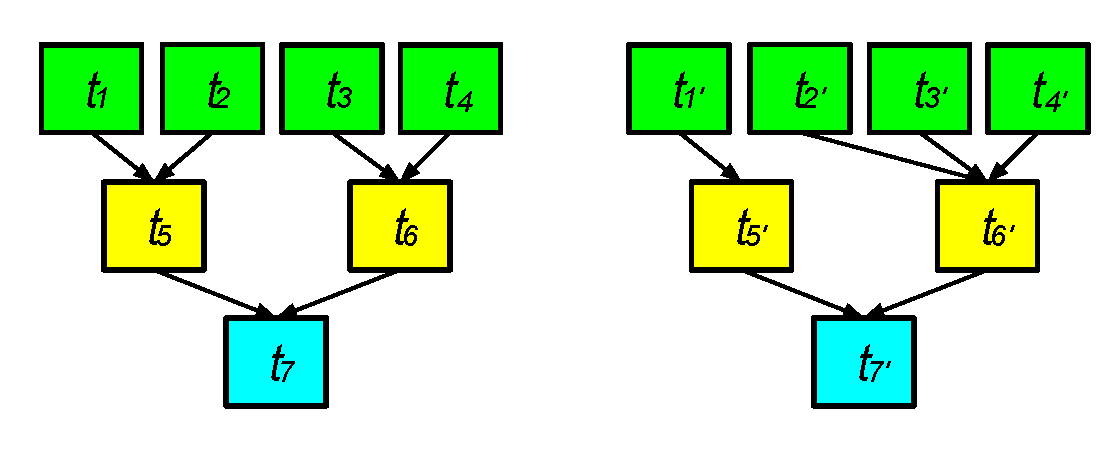
\includegraphics[width=0.85\linewidth]{figures/imbalance/dependency.pdf}
	\captionof{figure}{Example of workflows with different data dependencies (For better visualization, we do not show system overheads in the rest of the paper).}
	\label{fig:imbalance_hifv}
\end{figure}

\textbf{Distance Variance} ($DV$) describes how `close' tasks are to each other. The distance between two tasks/jobs is defined as the cumulative length of the path to their closest common successor. If they do not have a common successor, the distance is set to infinity. For a group of $n$ tasks/jobs, the distance between them is represented by a $n \times n$ matrix $D$, where an element $D(u,v)$ denotes the distance between a pair of tasks/jobs $u$ and $v$. For any workflow structure, $D(u,v)=D(v,u)$ and $D(u,u)=0$, thus we ignore the cases when $u \geq v$. Distance Variance is then defined as the standard deviation of all the elements $D(u,v)$ for $u<v$. The time complexity of calculating all the $D$ of a workflow with $n$ tasks is $O(n^2)$. 

Similarly, $HDV$ indicates the $DV$ of a group of tasks/jobs at the same horizontal level. For example, Table~\ref{tab:imblance_metric} shows the distance matrices of tasks from the first level for both workflows of Figure~\ref{fig:imbalance_hifv} ($D_1$ for the workflow in the left, and $D_2$ for the workflow in the right). $HDV$ for $t_1, t_2, t_3$, and $t_4$ is 1.03, and for $t_{1'}, t_{2'}, t_{3'}$, and $t_{4'}$ is 1.10. In terms of distance variance, $D_1$ is more `even' than $D_2$. A smaller $HDV$ means the tasks at the same horizontal level are more equally `distant' from each other and thus the workflow structure tends to be more `even' and `regular'. 

\begin{table}[htb]
	\footnotesize
	\centering
	\begin{tabular}{l|rrrr}
		$D_1$ & $t_1$ & $t_2$ & $t_3$ &$t_4$\\
		\hline
		$t_1$ & 0 & 2 & 4 & 4 \\
		$t_2$ & 2 & 0 & 4 & 4 \\
		$t_3$ & 4 & 4 & 0 & 2\\
		$t_4$ & 4 & 4 & 2 & 0 \\
	\end{tabular}
	\quad
	\begin{tabular}{l|rrrr}
		$D_2$ & $t_1'$ & $t_2'$ & $t_3'$ &$t_4'$\\
		\hline
		$t_1'$ & 0 & 4 & 4 & 4 \\
		$t_2'$ & 4 & 0 & 2 & 2 \\
		$t_3'$ & 4 & 2 & 0 & 2\\
		$t_4'$ & 4 & 2 & 2 & 0 \\
	\end{tabular}
	\caption{Distance matrices of tasks from the first level of workflows in Figure~\ref{fig:imbalance_hifv}.}
	\label{tab:imblance_metric}
\end{table}

In conclusion, runtime variance and dependency variance offer a quantitative and comparable tool to measure and evaluate the internal structure of a workflow. 



\subsection{Balanced clustering methods}
\label{sec:methods}
In this subsection, we introduce our balanced clustering methods used to improve the runtime and dependency balances in task clustering. We first introduce the basic runtime-based clustering method, and then two other balancing methods that address the dependency imbalance problem. %We use the metrics presented in the previous subsection to evaluate a given workflow to decide which balancing method(s) is(are) more appropriate. 

%Algorithm~\ref{alg:imbalance_algo} shows the pseudocode of our balanced clustering algorithm that uses a combination of these balancing methods and metrics.  The maximum number of clustered jobs (size of $CL$) is equal to the number of available resources multiplied by a \emph{clustering factor}. 

%\begin{algorithm}[htb]
%	\caption{ Balanced Clustering algorithm}
%	\footnotesize
%	\label{alg:imbalance_algo}
%	\begin{algorithmic}[1]
%		\Require $W$: workflow; $CL$: list of clustered jobs; $C$: the required size of $CL$; 
%		\Ensure The job runtime of $CL$ are as even as possible
%		\Procedure{Clustering}{$W,D,C$}
%			\State Sort $W$ in decreasing order of the size of each level
%			\For{$level < $the depth of $W$}
%				\State $TL\gets $\ \Call{GetTasksAtLevel}{$w,level$} \Comment{Partition $W$ based on depth}
%				\State $CL\gets$  \ \Call{Merge}{$TL,C$} \Comment{Form a list of clustered jobs}
%				\State $W \gets W - TL + CL$  \Comment{Merge dependencies as well} 
%			\EndFor
%		\EndProcedure
%		\Procedure{Merge}{$TL, C$}
%			\State Sort $TL$ in decreasing order of task runtime
%			\For{$t\ in\ TL$}
%				\State $J \gets $\ \Call{GetCandidateJob}{$CL, t$} \Comment{Get a candidate task}
%				\State  $J \gets J\ +\ t$ \Comment{Merge it with the clustered job}
%			\EndFor
%			\State \textbf{return} $CL$
%		\EndProcedure
%		\Procedure{GetCandidateJob}{$CL, t$}
%			\State Selects a job based on balanced clustering methods
%		\EndProcedure
%	\end{algorithmic}
%\end{algorithm}

%We examine tasks in a level-by-level approach starting from the level with the largest width (number of tasks at the same level, \texttt{line 2}). The intuition behind this breadth favored approach is that we believe it should improve the performance most. Then, we determine which type of imbalance problem a workflow experiences based on the balanced clustering metrics presented previously ($HRV$, $HIFV$, and $HDV$), and accordingly, we select a combination of balancing methods. \textsc{GetCandidateJob} selects a job (\texttt{line 12}) from a list of potential candidate jobs ($CL$) to be merged with the targeting task ($t$). Below we introduce the three balancing methods proposed in this work.


\begin{algorithm}[!htb]
	\footnotesize
	\caption{Horizontal Runtime Balancing algorithm.}
	\label{alg:imbalance_hrb}
	\begin{algorithmic}[1]
		\Require $W$: workflow; $C$: number of tasks per jobs; $R$: number of jobs per horizontal level
		\Procedure{Clustering}{$W,C$}
			\For{$level < depth(W)$}
				\State $TL\gets $\ \Call{GetTasksAtLevel}{$W,level$} \Comment{Partition $W$ based on depth}
				\State $CL\gets$  \ \Call{Merge}{$TL,C, R$} \Comment{Returns a list of clustered jobs}
				\State $W \gets W - TL + CL$  \Comment{Merge dependencies as well} 
			\EndFor
		\EndProcedure
		\Procedure{Merge}{$TL, C, R$}
			\For{$i<R$}
			\State $J_i\gets$\{\}\Comment{An empty job}
			\EndFor
			\State $CL\gets$\{\}\Comment{An empty list of clustered jobs}
			\State Sort $TL$ in descending of runtime
			\ForAll{$t$ in $TL$}
				\State $J\gets$ the job with shortest runtime and less than $C$ tasks  
				\State $J$.add ($t$) \Comment{Adds the task to the shortest job}
				
			\EndFor
			\For{$i<R$}
			\State  $CL$.add( $J_i$)
			\EndFor
			\State \textbf{return} $CL$
		\EndProcedure
	\end{algorithmic}
\end{algorithm}



\textbf{Horizontal Runtime Balancing} (HRB) aims to evenly distribute task runtime among clustered jobs. Tasks with the longest runtime are added to the job with the shortest runtime. Algorithm~\ref{alg:imbalance_hrb} shows the pseudo codes of HRB. This greedy method is used to address the load balance problem caused by runtime variance at the same horizontal level. Figure~\ref{fig:imbalance_hrb} shows an example of HRB where tasks in the first level have different runtimes and should be grouped into two jobs. HRB sorts tasks in decreasing order of runtime, and then adds the task with the highest runtime to the group with the shortest aggregated runtime. Thus, $t_1$ and $t_3$, as well as $t_2$ and $t_4$ are merged together.
For simplicity, system overheads are not displayed.


\begin{algorithm}[!htb]
	\footnotesize
	\caption{Horizontal Impact Factor Balancing algorithm.}
	\label{alg:imbalance_hifb}
	\begin{algorithmic}[1]
		\Require $W$: workflow; $C$: number of tasks per jobs; $R$: number of jobs per horizontal level
		\Procedure{Clustering}{$W,C$}
			\For{$level < depth(W)$}
				\State $TL\gets $\ \Call{GetTasksAtLevel}{$W,level$} \Comment{Partition $W$ based on depth}
				\State $CL\gets$  \ \Call{Merge}{$TL,C, R$} \Comment{Returns a list of clustered jobs}
				\State $W \gets W - TL + CL$  \Comment{Merge dependencies as well} 
			\EndFor
		\EndProcedure
		\Procedure{Merge}{$TL, C, R$}
			\For{$i<R$}
			\State $J_i\gets$\{\}\Comment{An empty job}
			\EndFor
			\State $CL\gets$\{\}\Comment{An empty list of clustered jobs}
			\State Sort $TL$ in descending of runtime
			\ForAll{$t$ in $TL$}
				\State $L\gets$ Sort all $J_i$ with the similarity of impact factors with $t$
				\State $J\gets$ the job with shortest runtime and less than $C$ tasks in $L$
				\State $J$.add ($t$) 
				
			\EndFor
			\For{$i<R$}
			\State  $CL$.add( $J_i$)
			\EndFor
			\State \textbf{return} $CL$
		\EndProcedure
	\end{algorithmic}
\end{algorithm}


\begin{algorithm}[!htb]
	\footnotesize
	\caption{Horizontal Distance Balancing algorithm.}
	\label{alg:imbalance_hdb}
	\begin{algorithmic}[1]
		\Require $W$: workflow; $C$: number of tasks per jobs; $R$: number of jobs per horizontal level
		\Procedure{Clustering}{$W,C$}
			\For{$level < depth(W)$}
				\State $TL\gets $\ \Call{GetTasksAtLevel}{$W,level$} \Comment{Partition $W$ based on depth}
				\State $CL\gets$  \ \Call{Merge}{$TL,C, R$} \Comment{Returns a list of clustered jobs}
				\State $W \gets W - TL + CL$  \Comment{Merge dependencies as well} 
			\EndFor
		\EndProcedure
		\Procedure{Merge}{$TL, C, R$}
			\For{$i<R$}
			\State $J_i\gets$\{\}\Comment{An empty job}
			\EndFor
			\State $CL\gets$\{\}\Comment{An empty list of clustered jobs}
			\State Sort $TL$ in descending of runtime
			\ForAll{$t$ in $TL$}
				\State $L\gets$ Sort all $J_i$ with the closest distance with $t$
				\State $J\gets$ the job with shortest runtime and less than $C$ tasks in $L$
				\State $J$.add ($t$) 
				
			\EndFor
			\For{$i<R$}
			\State  $CL$.add( $J_i$)
			\EndFor
			\State \textbf{return} $CL$
		\EndProcedure
	\end{algorithmic}
\end{algorithm}


%how HRB works in an example of four jobs with different job runtime (assuming the height of a job is its runtime). For the given task ($t_0$), HRB sorts the potential jobs ($j_1$, $j_2$, $j_3$, and $j_4$) based on their runtime and selects the shortest job (in this case $j_1$ or $j_2$). 

\begin{figure}[htb]
	\centering
	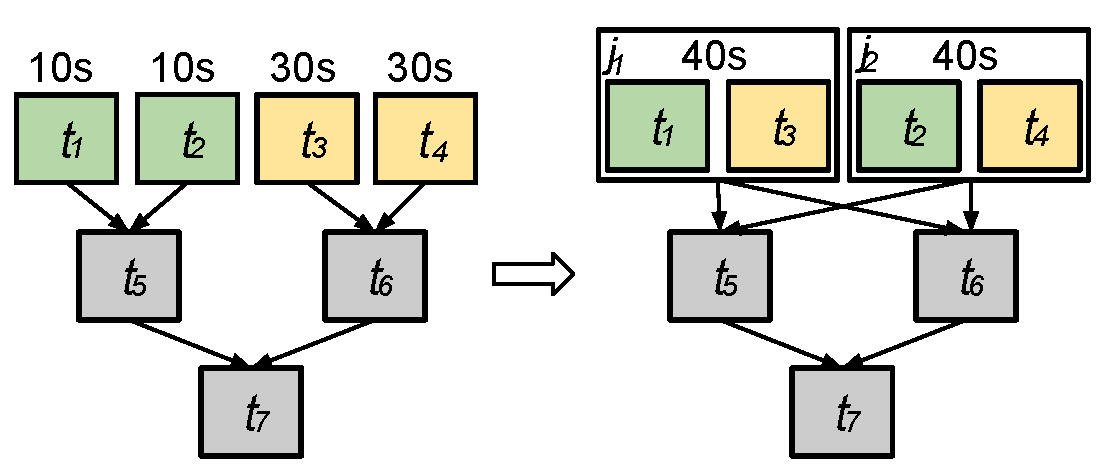
\includegraphics[width=0.85\linewidth]{figures/imbalance/hrb.pdf}
	\caption{An example of the HRB (Horizontal Runtime Balancing) method. By solely addressing runtime variance, data locality problems may arise.}
	\label{fig:imbalance_hrb}
\end{figure}

However, HRB may cause a dependency imbalance problem since the clustering does not take data dependency into consideration. To address this problem, we propose the \textbf{Horizontal Impact Factor Balancing} (HIFB) and the \textbf{Horizontal Distance Balancing} (HDB) methods. 

In HRB, candidate jobs within a workflow level are sorted by their runtime, while in HIFB jobs are first sorted based on their similarity of $IF$, then on runtime. 
Algorithm~\ref{alg:imbalance_hifb} shows the pseudo codes of HIFB. 
For example, in Figure~\ref{fig:imbalance_hifb}, $t_1$ and $t_2$ have $IF = 0.25$, while $t_3$, $t_4$, and $t_5$ have $IF = 0.16$. HIFB selects a list of candidate jobs with the same IF value, and then HRB is performed to select the shortest job. Thus, HIFB merges $t_1$ and $t_2$ together, as well as $t_3$ and $t_4$.

\begin{figure}[htb]
	\centering
	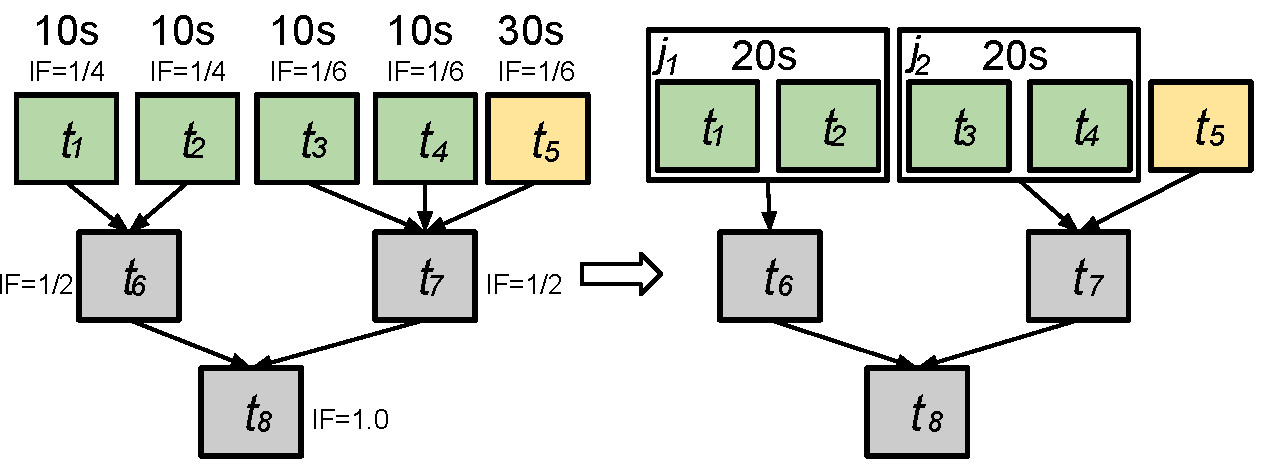
\includegraphics[width=\linewidth]{figures/imbalance/hifb.pdf}
	\captionof{figure}{An example of the HIFB (Horizontal Impact Factor Balancing) method. Impact factors allow the detection of similarities between tasks.}
	\label{fig:imbalance_hifb}
\end{figure}

However, HIFB is suitable for workflows with asymmetric structure. For symmetric workflows, such as the one shown in Figure~\ref{fig:imbalance_hrb}, the $IF$ value for all tasks of the first level will be the same ($IF=0.25$), thus the method may also cause dependency imbalance. In HDB, jobs are sorted based on the distance between them and the targeted task $t$, then on their runtimes. 
Algorithm~\ref{alg:imbalance_hdb} shows the pseudo codes of HDB. 
For instance, in Figure~\ref{fig:imbalance_hdb}, the distances between tasks $D(t_1,t_2)=D(t_3,t_4)=2$, while $D(t_1,t_3)=D(t_1,t_4)=D(t_2,t_3)=D(t_2,t_4)=4$. Thus, HDB merges a list of candidate tasks with the minimal distance ($t_1$ and $t_2$, and $t_3$ and $t_4$). Note that even if the workflow is asymmetric (Figure~\ref{fig:imbalance_hifb}), HDB would obtain the same result as with HIFB. 

\begin{figure}[!htb]
	\centering
	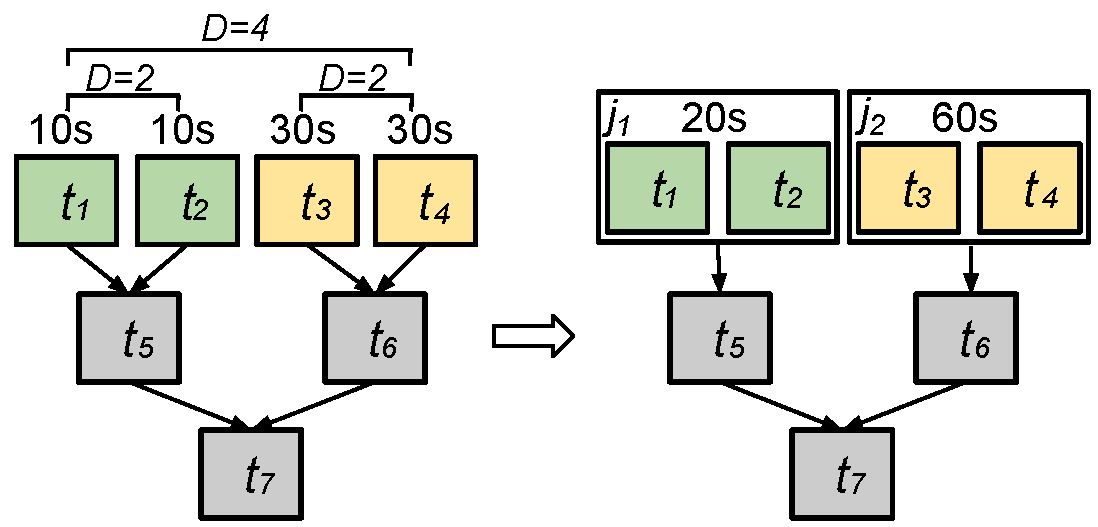
\includegraphics[width=0.85\linewidth]{figures/imbalance/hdb.pdf}
	\captionof{figure}{An example of the HDB (Horizontal Distance Balancing) method. Measuring the distances between tasks avoids data locality problems.}
	\label{fig:imbalance_hdb}
\end{figure}

There are cases where HDB would yield lower performance than HIFB. For instance, let $t_1$, $t_2$, $t_3$, $t_4$, and $t_5$ be the set of tasks to be merged in the workflow presented in Figure~\ref{fig:imbalance_hifb_hdb}. HDB does not identify the difference in the number of parent/child tasks between the tasks, since $d(t_u,t_v) = 2, \forall u,v \in [1,5], u \neq v$. On the other hand, HIFB does distinguish them since their impact factors are slightly different. Example of such scientific workflows include the LIGO Inspiral workflow~\cite{LIGO}, which is used in the evaluation of this work (Section~\ref{sec:results}).

\begin{figure}[!htb]
	\centering
	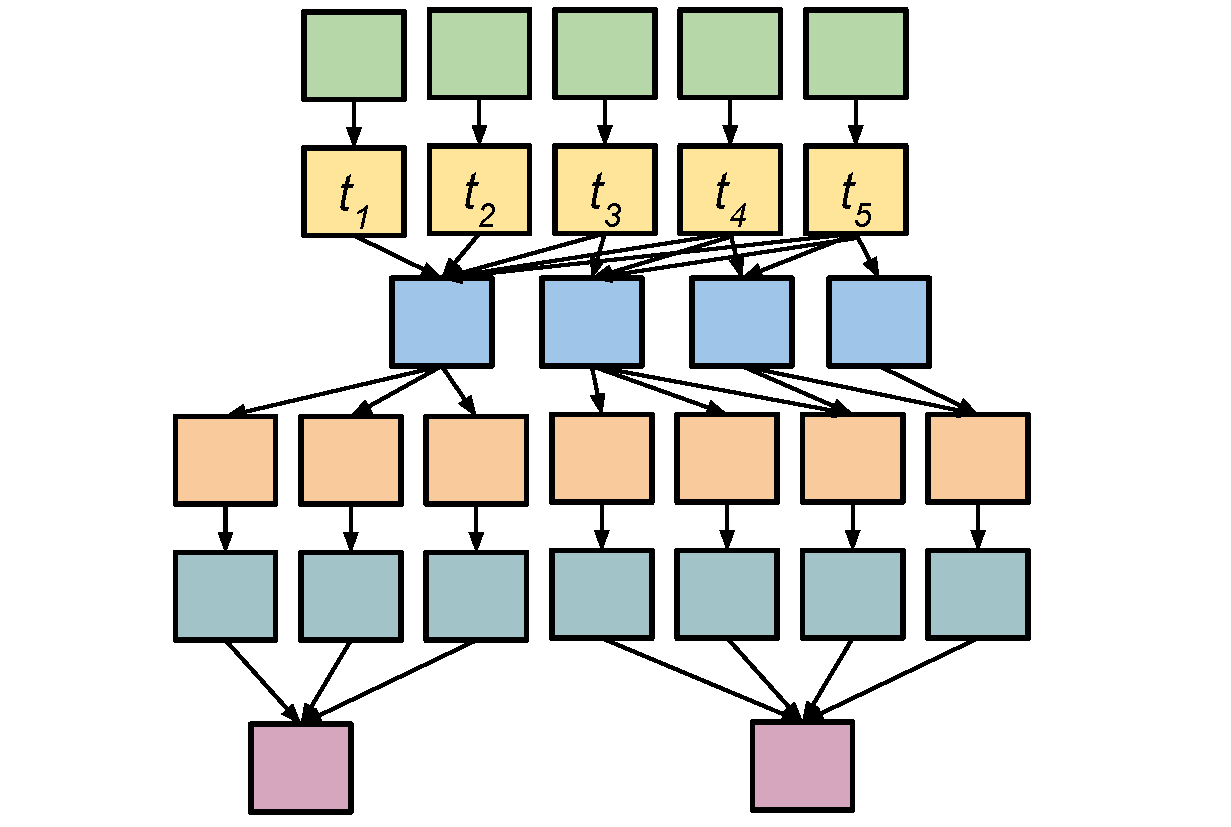
\includegraphics[width=0.85\linewidth]{figures/imbalance/hifb_vs_hdb.pdf}
	\captionof{figure}{A workflow example where HDB yields lower performance than HIFB. HDB does not capture the difference in the number of parents/child tasks, since the distances between tasks ($t_1$, $t_2$, $t_3$, $t_4$, and $t_5$) are the same.}
	\label{fig:imbalance_hifb_hdb}
\end{figure}

%In conclusion, these balancing methods have different preference on the selection of a candidate job to be merged with the targeting task. HIFB tends to group tasks that share similar position/importance to the workflow structure. HDB tends to group tasks that are closed to each other to reduce data transfers. 
Table~\ref{tab:2} summarizes the imbalance metrics and balancing methods presented in this work. 

\begin{figure}[htb]
	\centering
	\small
	\begin{tabular}{l|l}
		\hline
		\textbf{Imbalance Metrics} & $abbr.$   \\
		\hline
		Horizontal Runtime Variance & \emph{HRV}   \\ 
%		%Pipeline Runtime Variance &{\em PRV}  \\ 
		Horizontal Impact Factor Variance & \emph{HIFV} \\ 
		Horizontal Distance Variance & \emph{HDV}  \\ 
		\hline
		\textbf{Balancing Methods} & $abbr.$  \\
		\hline
%		Horizontal Clustering & HC \\
		Horizontal Runtime Balancing & HRB   \\ 
%		Vertical Clustering & VC \\ 
		Horizontal Impact Factor Balancing & HIFB\\ 
		Horizontal Distance Balancing & HDB \\ 
		\hline
	\end{tabular}
	\captionof{table}{Summary of imbalance metrics and balancing methods.}
	\label{tab:2}
\end{figure}



\subsection{Combining vertical clustering methods}

In this subsection, we discuss how we combine the balanced clustering methods presented above with vertical clustering (VC).
%For one example workflow shown in Figure~\ref{fig:imbalance_vc}, we may simply merge tasks at the fourth level and tasks at the fifth level vertically. 
In pipelined workflows (single-parent-single-child tasks), vertical clustering always yields improvement over a baseline, non-clustered execution because the merging reduces system overheads and data transfers within the pipeline. Horizontal clustering does not have the same guarantee since its performance depends on the comparison of system overheads and task durations. However, vertical clustering has limited performance improvement if the workflow does not have pipelines. Therefore, we are interested in the analysis of the performance impact of applying both vertical and horizontal clustering in the same workflow. We combine these methods in two ways: (\emph{i}) \emph{VC-prior}, and (\emph{ii}) \emph{VC-posterior}.


%\label{sec:vertical}
%\begin{figure}[htb]
%	\centering
%	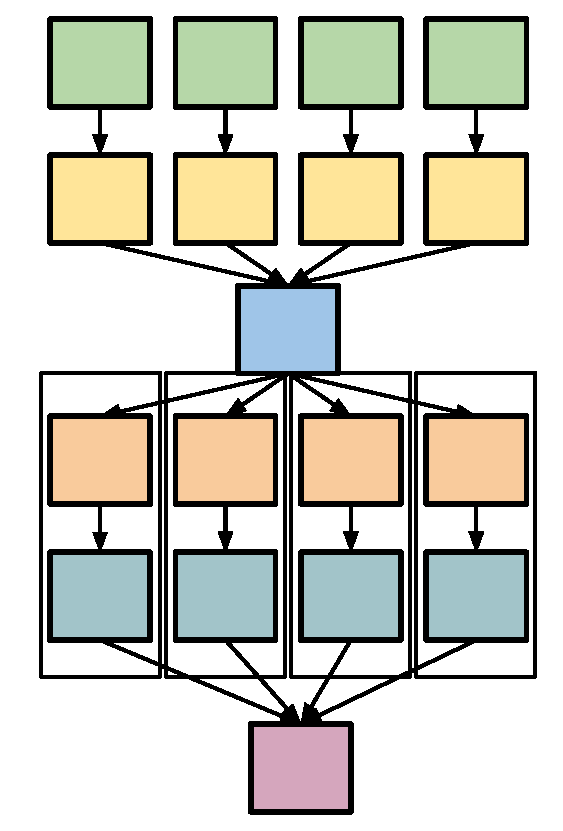
\includegraphics[width=0.35\linewidth]{figures/imbalance/vertical_clustering.pdf}
%	\captionof{figure}{An example of Vertical Clustering.}
%	\label{fig:imbalance_vc}
%\end{figure}

\paragraph{\textbf{VC-prior}}
In this method, vertical clustering is performed first, and then the balancing methods (HRB, HIFB, HDB, or HC) are applied. Figure~\ref{fig:imbalance_vc_prior} shows an example where pipelined-tasks are merged first, and then the merged pipelines are horizontally clustered based on the runtime variance.

\begin{figure}[!htb]
	\centering
	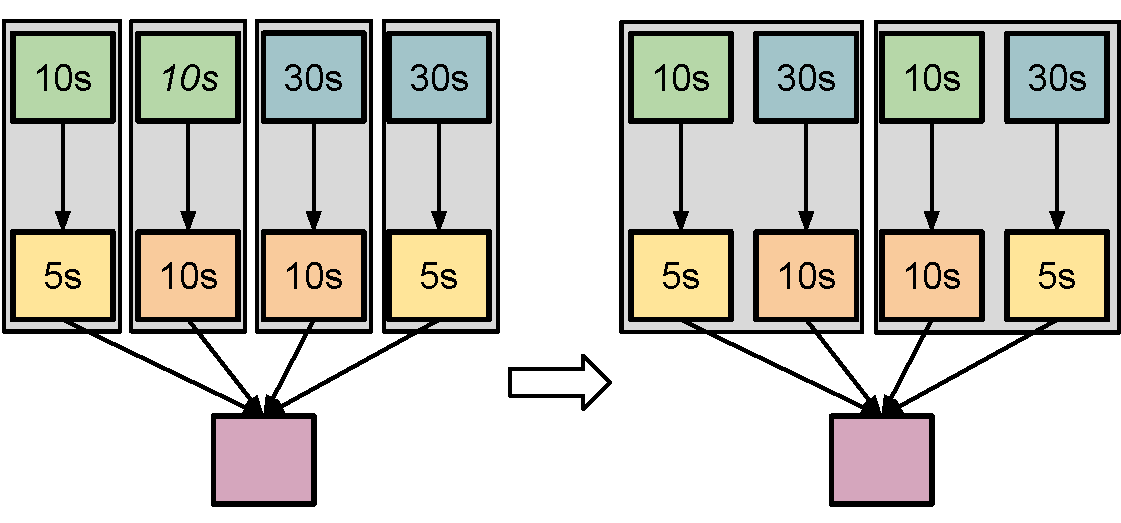
\includegraphics[width=0.85\linewidth]{figures/imbalance/vertical_clustering_prior.pdf}
	\captionof{figure}{\emph{VC-prior}: vertical clustering is performed first, and then the balancing methods.}
	\label{fig:imbalance_vc_prior}
\end{figure}

\paragraph{\textbf{VC-posterior}} 
%Here, vertical clustering is performed \emph{a posteriori}, i.e. balancing methods are first applied, and then VC. Figure~\ref{fig:imbalance_vc_posterior} shows an example where tasks are horizontally clustered first based on the runtime variance, and then merged vertically. In this example, vertical clustering targeted the data locality problem by merging tasks that would not generate interdependency once clustered. However, this approach causes a runtime imbalance problem.

\begin{figure}[!htb]
	\centering
	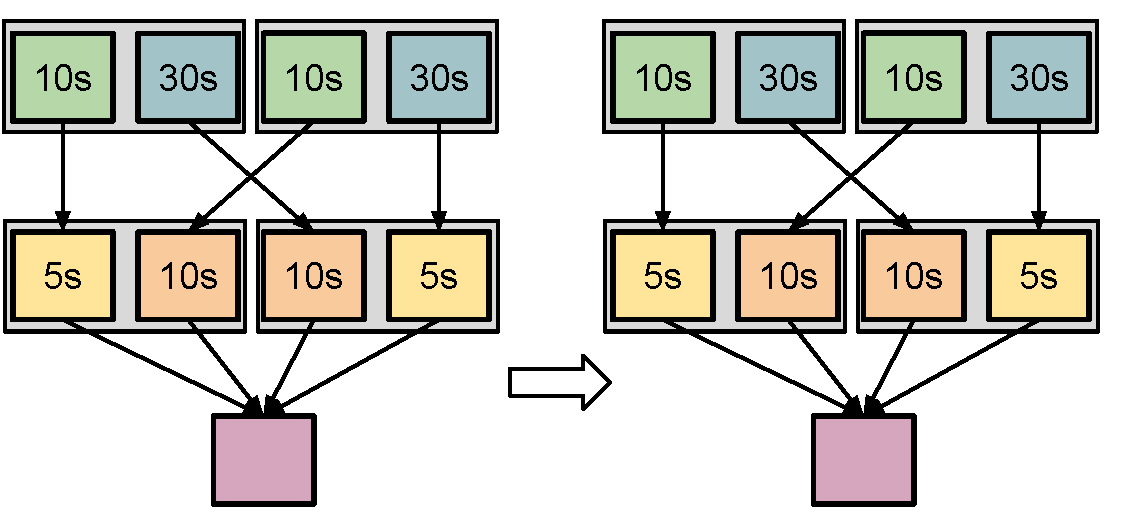
\includegraphics[width=0.85\linewidth]{figures/imbalance/vertical_clustering_posterior3.pdf}
	\captionof{figure}{\emph{VC-posterior}: horizontal clustering (balancing methods) is performed first, and then vertical clustering.}
	\label{fig:imbalance_vc_posterior}
\end{figure}

Here, balancing methods are first applied, and then vertical clustering. Figure~\ref{fig:imbalance_vc_posterior} shows an example where tasks are horizontally clustered first based on the runtime variance, and then merged vertically. However, since the original pipeline structures have been broken by horizontal clustering, VC does not perform any changes to the workflow. 


%means we perform horizontal clustering methods first and then vertical clustering. For the same workflow, assuming we merge tasks horizontally as shown in , we can see that we cannot perform vertical clustering to clustered jobs at the fourth level and the fifth level since the original pipeline structures have been destroyed by horizontal clustering. This phenomenon suggests us VC-posterior may work better compared to VC-prior, generally speaking. However, some opposite cases do exist. We will verify our hypothesis in Section~\ref{sec:results}. We will also compared the two combining approaches with \textbf{VC-only}, which means we perform vertical clustering only and \textbf{No-VC}, which means we just perform horizontal clustering methods without vertical clustering. 







% Section
\section{Evaluation}
\label{sec:experiments}

The experiments presented hereafter evaluate the performance of our balancing methods when compared to an existing and effective task clustering strategy named Horizontal Clustering (HC)~\cite{Singh:2008:WTC:1341811.1341822}, which is widely used by workflow management systems such as Pegasus. We also compare our methods with two legacy heuristics from the literature: DFJS~\cite{Muthuvelu:2005:DJG:1082290.1082297}, and AFJS~\cite{Liu2009}. DFJS groups bag of tasks based on the �task durations up to the resource capacity. AFJS is an extended version of DFJS that is an adaptive fine-grained job scheduling algorithm to group fine-grained tasks according to processing capacity and bandwidth of the current available resources.

% Workflow applications
\subsection{Scientific workflow applications}
\label{sec:applications}

Five real scientific workflow applications are used in the experiments: LIGO~\cite{LIGO} Inspiral analysis, Montage~\cite{Berriman2004}, CyberShake~\cite{Graves2010}, Epigenomics~\cite{Epigenome}, and SIPHT~\cite{SIPHT}. 

\paragraph{\textbf{LIGO}}
The Laser Interferometer Gravitational Wave Observatory (LIGO) workflows are used to search for gravitational wave signatures in data collected by large-scale interferometers. The observatories' mission is to detect and measure gravitational waves predicted by general relativity ��Einstein's theory of gravity �in which gravity is described as due to the curvature of the fabric of time and space. LIGO Inspiral workflow is a data intensive workflow. Figure~\ref{fig:evaluation_shape_ligo} shows a simplified version of the workflow.

\begin{figure}[!htb]
	\centering
	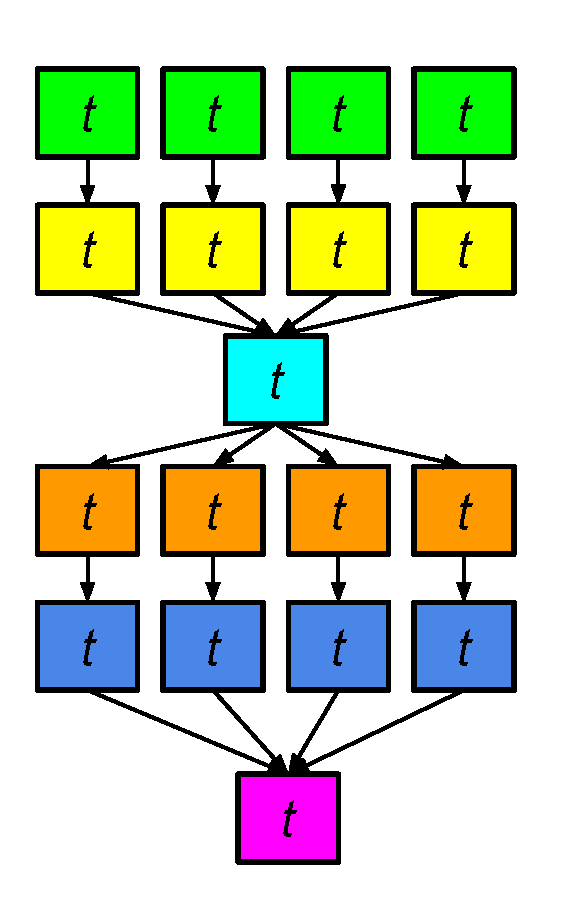
\includegraphics[width=0.6\linewidth]{figures/evaluation/inspiral.pdf} \\
	\caption{A simplified visualization of the LIGO Inspiral workflow.}
	\label{fig:evaluation_shape_ligo}
\end{figure}

\paragraph{\textbf{Montage}}
Montage is an astronomy application that is used to construct large image mosaics of the sky. Input images are reprojected onto a sphere and overlap is calculated for each input image. The application re-projects input images to the correct orientation while keeping background emission level constant in all images. The images are added by rectifying them into a common flux scale and background level. Finally the reprojected images are co- added into a final mosaic. The resulting mosaic image can provide a much deeper and detailed understanding of the portion of the sky in question. Figure~\ref{fig:evaluation_shape_montage} illustrates a small Montage workflow. The size of the workflow depends on the number of images used in constructing the desired mosaic of the sky. The structure of the workflow changes to accommodate increases in the number of inputs, which corresponds to an increase in the number of computational tasks.



\begin{figure}[htb]
	\centering
	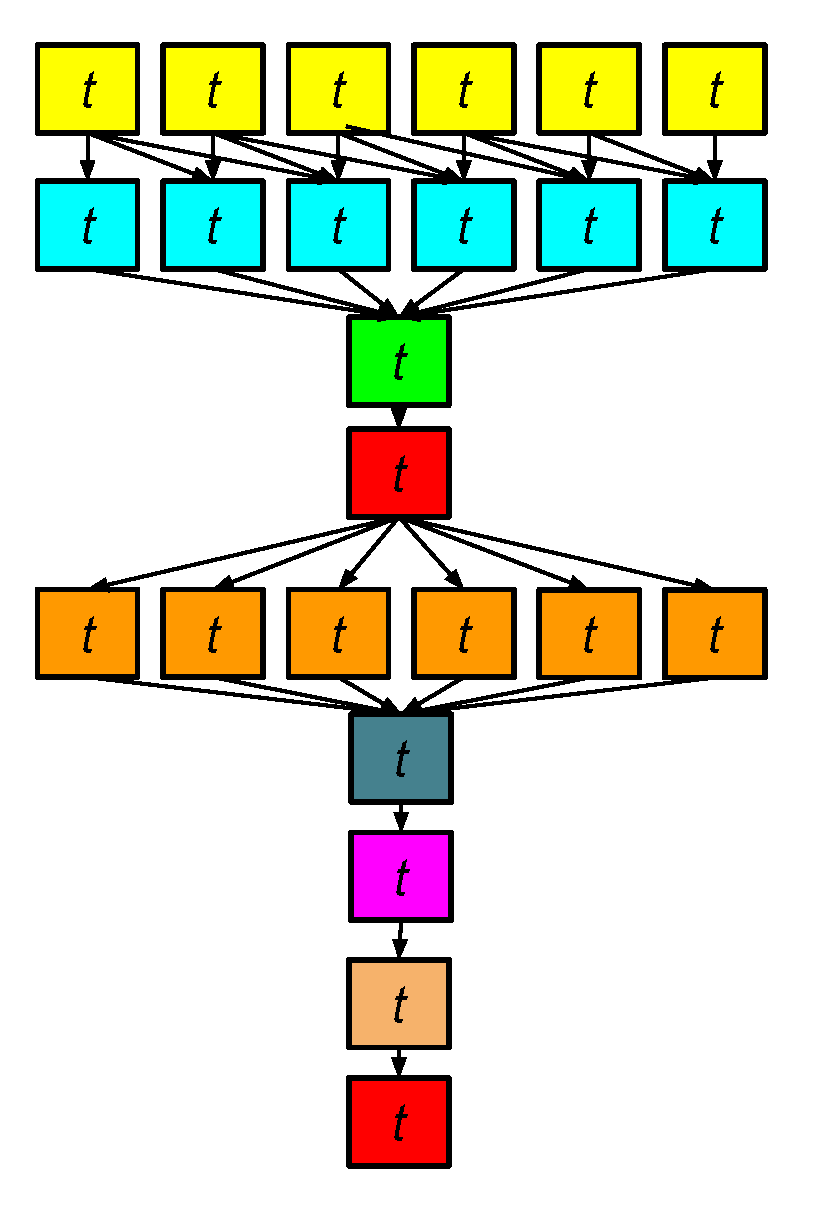
\includegraphics[width=0.55\linewidth]{figures/evaluation/montage.pdf} \\
	\caption{A simplified visualization of the Montage workflow.}
	\label{fig:evaluation_shape_montage}
\end{figure}

\paragraph{\textbf{Cybershake}}
CyberShake is a seismology application that calculates Probabilistic Seismic Hazard curves for geographic sites in the Southern California region. It identifies all ruptures within 200km of the site of interest and convert rupture definition into multiple rupture variations with differing hypocenter locations and slip distributions. It then calculates synthetic seismograms for each rupture variance and peak intensity measures are then extracted from these synthetics and combined with the original rupture probabilities to produce probabilistic seismic hazard curves for the site. Figure~\ref{fig:evaluation_shape_cybershake} shows an illustration of the Cybershake workflow.

\begin{figure}[htb]
	\centering
	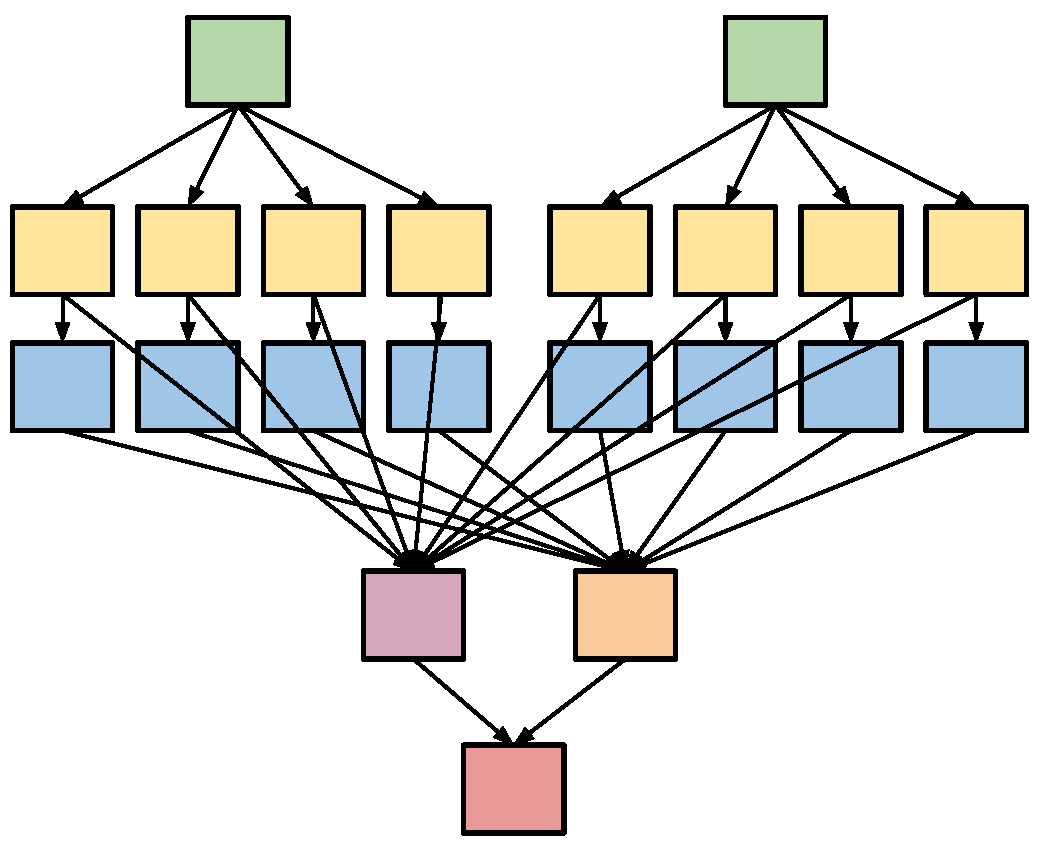
\includegraphics[width=0.7\linewidth]{figures/evaluation/cybershake.pdf} \\
	\caption{A simplified visualization of the CyberShake workflow.}
	\label{fig:evaluation_shape_cybershake}
\end{figure}

\paragraph{\textbf{Epigenomics}}
The Epigenomics workflow is a pipeline workflow. Initial data are acquired from the Illumina-Solexa Genetic Analyzer in the form of DNA sequence lanes. Each Solexa machine can generate multiple lanes of DNA sequences. These data are converted into a format that can be used by sequence mapping software. The mapping software can do one of two major tasks. It either maps short DNA reads from the sequence data onto a reference genome, or it takes all the short reads, treats them as small pieces in a puzzle and then tries to assemble an entire genome. In our experiments, the workflow maps DNA sequences to the correct locations in a reference Genome. This generates a map that displays the sequence density showing how many times a certain sequence expresses itself on a particular location on the reference genome. Scientists draw conclusions from the density of the acquired sequences on the reference genome. Epigenome is a CPU-intensive application and its simplified structure is shown on Figure~\ref{fig:evaluation_shape_genome}. 

\begin{figure}[htb]
	\centering
	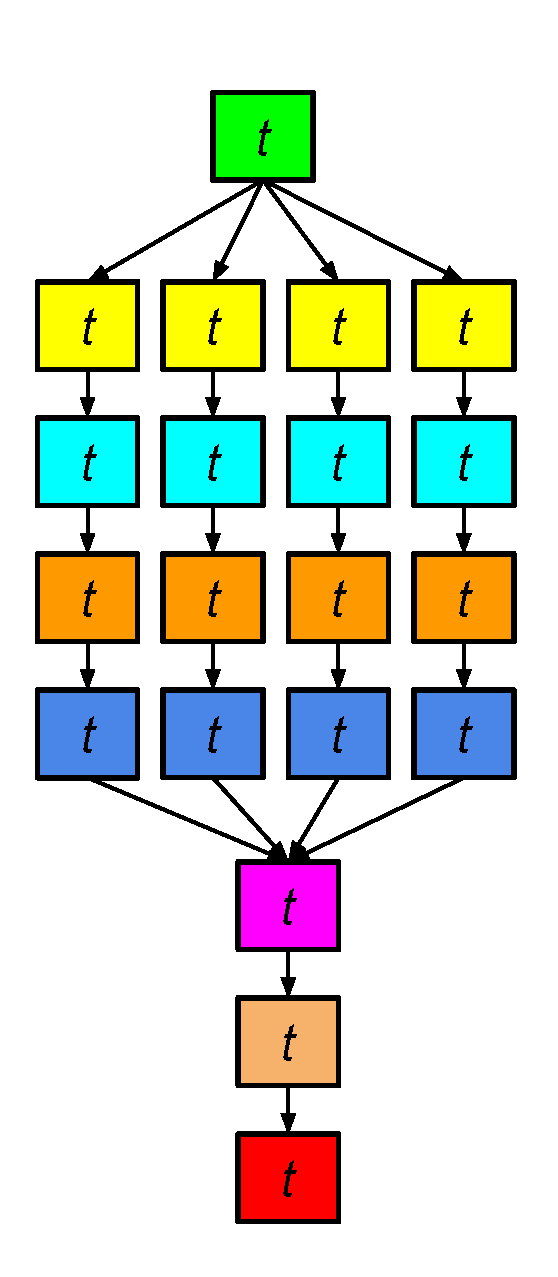
\includegraphics[width=\linewidth]{figures/evaluation/genome.pdf} \\
	\caption{A simplified visualization of the Epigenomics workflow.}
	\label{fig:evaluation_shape_genome}
\end{figure}

\paragraph{\textbf{SIPHT}}
The SIPHT workflow is conducting a wide search for small untranslated RNAs (sRNAs) that regulate several processes such as secretion or virulence in bacteria. The kingdom-wide prediction and annotation of sRNA encoding genes involves a variety of individual programs that are executed in the proper order using PEGASUS. These involve the prediction of Rho-independent transcriptional terminators, BLAST (Basic Local Alignment Search Tools) comparisons of the inter genetic regions of different replicons and the annotations of any sRNAs that are found. A simplified structure of the SIPHT workflow is shown on Figure~\ref{fig:evaluation_shape_sipht}. 

\begin{figure}[htb]
	\centering
	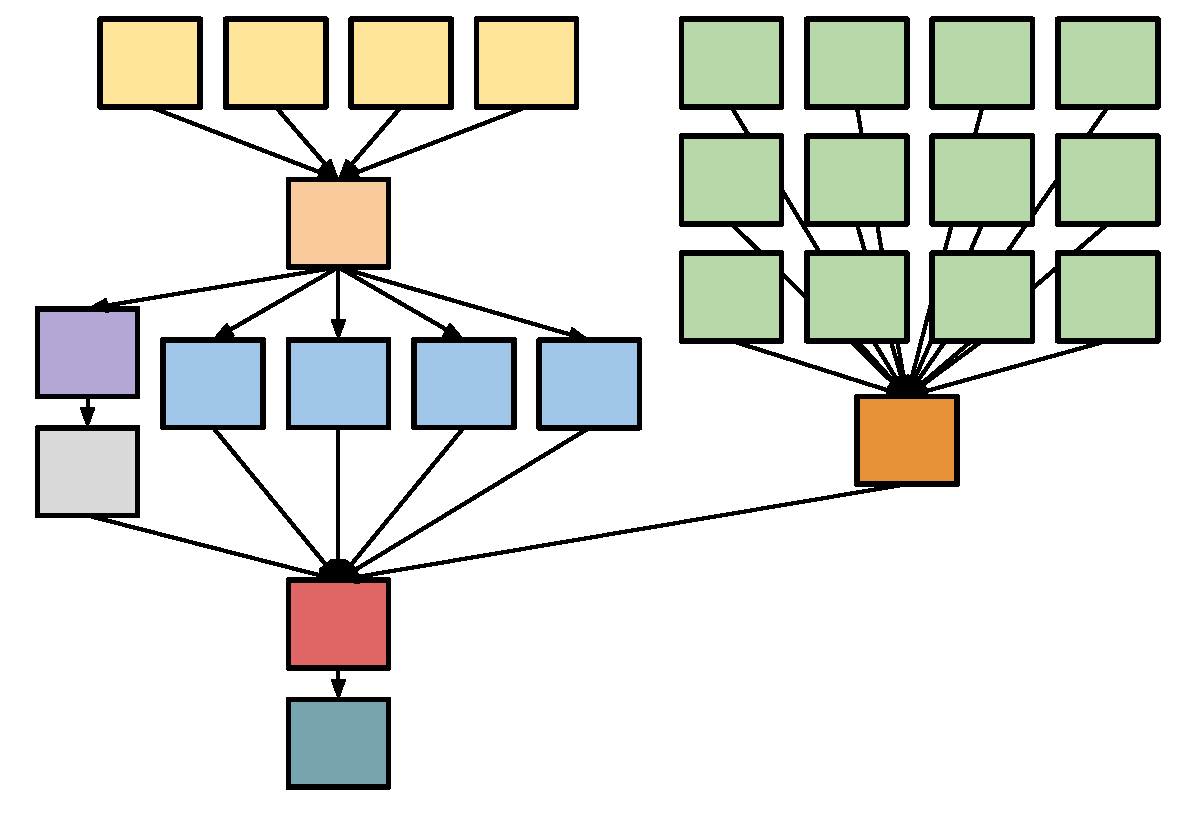
\includegraphics[width=0.7\linewidth]{figures/evaluation/sipht.pdf} \\
	\caption{A simplified visualization of the SIPHT workflow.}
	\label{fig:evaluation_shape_sipht}
\end{figure}

Table~\ref{tab:evaluation_workflows} shows the summary of the main workflows characteristics: number of tasks, average data size, and average task runtimes. 

\begin{table}[!htb]
	\centering
	\small
	\begin{tabular}{lrrrr}
		\hline
		Workflow & Tasks & Avg. Data Size &  Avg. Task Runtime \\
		\hline
		LIGO 		&800		& 5 MB	&228s\\
		Montage 		&300		&3 MB	&11s\\
		CyberShake 	&700		&148 MB 	& 23s\\
		Epigenomics 	&165 	& 355 MB	&2952s\\
		\hline
	\end{tabular}
	\caption{Summary of the scientific workflows characteristics.}
	\label{tab:evaluation_workflows}
\end{table} 
\note{Add information for SIPHT in the table.}



% Task clustering techniques
\subsection{Task clustering techniques}

In the experiments, we compare the performance of our methods to the Horizontal Clustering (HC)~\cite{Singh:2008:WTC:1341811.1341822} technique, which is widely used by Pegasus, and with two methods from the literature, DFJS~\cite{Muthuvelu:2005:DJG:1082290.1082297} and AFJS~\cite{Liu2009}.

\paragraph{\textbf{HC}}
The Horizontal Clustering (HC) algorithm...
\note{Briefly explain the algorithm and add a pseudo-code.}

\paragraph{\textbf{DFJS}}
The dynamic fine-grained job scheduler (DFJS)...
\note{Briefly explain the algorithm and add a pseudo-code.}

\paragraph{\textbf{AFJS}}
The adaptive fine-grained job scheduler (AFJS)...
\note{Briefly explain the algorithm and add a pseudo-code.}

DFJS and AFJS require parameter tuning (e.g. resource capability) to efficiently cluster tasks into coarse-grained jobs. For instance, if the resource capacity is too high, all tasks may be grouped together, leading to loss of parallelism. In contrast, if it is too low, the algorithms do not group tasks, leading to no improvement over a control execution. For the comparison purposes of this work, we perform a parameter sweep study in order to optimize the algorithms for each workflow application described in Section~\ref{sec:applications}. However, explore all possible parameter combinations is a cumbersome and exhaustive task. Instead, we performed Binary Search...
\note{Briefly describe how did you perform the binary search.}

For simplicity, we use DFJS* and AFJS* to indicate their best searched performance in the rest of this work.

%In practice, these algorithms are not feasible to use since parameter tuning requires a lot of prior knowledge and it takes much time to search the parameter space without proper heuristics. . 


% Experiment conditions
\subsection{Experiment conditions}
We adopt a trace-based simulation approach, where we extended the WorkflowSim~\cite{Chen2012a} simulator with the balanced clustering methods and imbalance metrics to simulate a controlled distributed environment. \note{Add a sentence about WorkflowSim.} The simulated computing platform is composed by 20 single homogeneous core virtual machines (worker nodes), which is the quota per user of some typical distributed environments such as Amazon EC2~\cite{AmazonAWS} and FutureGrid~\cite{FutureGrid}. Amazon EC2 is a commercial, public cloud that is been widely used in distributed computing, in particular for scientific workflows~\cite{Juve09scientificworkflow}. FutureGrid is a distributed, high-performance testbed that provides scientists with a set of computing resources to develop parallel, grid, and cloud applications. Each simulated VM has 512MB of memory and the capacity to process 1,000 million instructions per second. Task scheduling algorithm is data-aware, i.e. tasks are scheduled to resources which have the most input data available.

We collected workflow execution traces~\cite{Chen2011, Juve2013} (including overhead and task runtime information) from real runs (executed on FutureGrid and Amazon EC2) of the scientific workflow applications described in Section~\ref{sec:applications}. The traces are used to fill the Workflow Generator toolkit~\cite{WorkflowGenerator} to generate synthetic workflows to perform simulations with several different configurations under controlled conditions. The toolkit uses the information gathered from actual scientific workflow executions to generate synthetic workflows resembling those used by real world scientific applications. The number of inputs to be processed, the number of tasks in the workflow, and their composition determine the structure of the generated workflow.

Three sets of experiments are conducted. Experiment 1 evaluates the performance gain ($\mu$) of our balancing methods (HRB, HIFB, and HDB) over a control execution (No Clustering). The goal of the experiment is to identify conditions where each method work best and worst. In addition, we also evaluate the performance gain of using workflow structure metrics (HRV, HIFV, and HDV), which require less \emph{a-priori} knowledge from task and resource characteristics, over task clustering techniques from the literature (HC, DFJS*, and AFJS*).
%Since DFJS requires one parameter (resource capacity) and AFJS requires two parameters (resource capacity and bandwidth capacity), we search all possible parameters to use their optimal performance gain. In practice, their performance should be equal to or lower than the optimal values. 

Experiment 2 evaluates the performance impact of the variation of average data size and the number of resources available in our balancing methods for one scientific workflow application (LIGO). The original average data size (both input and output data) of the LIGO workflow is about 5MB as shown in Table~\ref{tab:evaluation_workflows}. In this experiment, we increase the average data size up to 500MB to study the behavior of data intensive workflows.

Experiment 3 evaluates the influence of combining our horizontal clustering methods with vertical clustering. We compare the performance gain under four scenario, VC-prior: we perform VC first and then HIFB, HDB, HDB or HDC; VC-posterior: we perform horizontal methods and then VC; no VC: horizontal methods only; and VC only. The motivation behind this experiment is that we believe VC will change imbalance metrics (HIFV, HDV and HRV) and we aim to show how these metrics can help us understand the performance of VC better. 

%With these traces based information, we use WorkflowSim to vary algorithms used, resources, workflow size etc. to illustrate the different runtime performance of these methods. 
%Runtime (average and task runtime distribution) and overhead (workflow engine delay, queue delay, and network bandwidth) information were collected from real traces production environments~\cite{Chen2011, Juve2013}, then used as input parameters for the simulations. 
%where we could evaluate the performance of our methods when varying the average data size and task runtime.



% Results and discussion
\subsection{Results and discussion}

\paragraph{\textbf{Experiment 1}}
Fig.~\ref{fig:evaluation_algorithm}  shows the performance gain over No Clustering (NC) $\mu$ of the balancing methods for the five workflows. We have a few conclusions from Fig.~\ref{fig:evaluation_algorithm}: (1). In general, all of these horizontal clustering methods improve the runtime performance significantly (up to 48\%) except for the case using HIFB in Epigenomics. The reason is that each branch of Epigenomics happen to have the same number of pipelines as Fig.~\ref{fig:evaluation_shape_big_genome} shows. In such case, the IFs of each task at the same horizontal level is the same and thus the HIFB cannot distinguish tasks and their dependency variance as shown in Table.~\ref{tab:evaluation_genome}. 
(2). Among the four workflows, we see more significant improvement for the CyberShake workflow and the Montage workflow compared to Epigenomics and LIGO. The reason is Epigenomics and LIGO have a relatively short task runtime compared to the system overheads and task clustering can significantly improve the overall runtime. 
(3). Among the five methods, in most of the cases, it is clear that our methods (HIFB, HDB and HRB) perform better than HC, DFJS* and AFJS*. The reason is that they don't take the runtime variance and dependency variance into consideration. As to the comparison among HIFB, HDB and HRB, we will show in Experiment 2. 

\begin{figure}[htb]
	\centering
	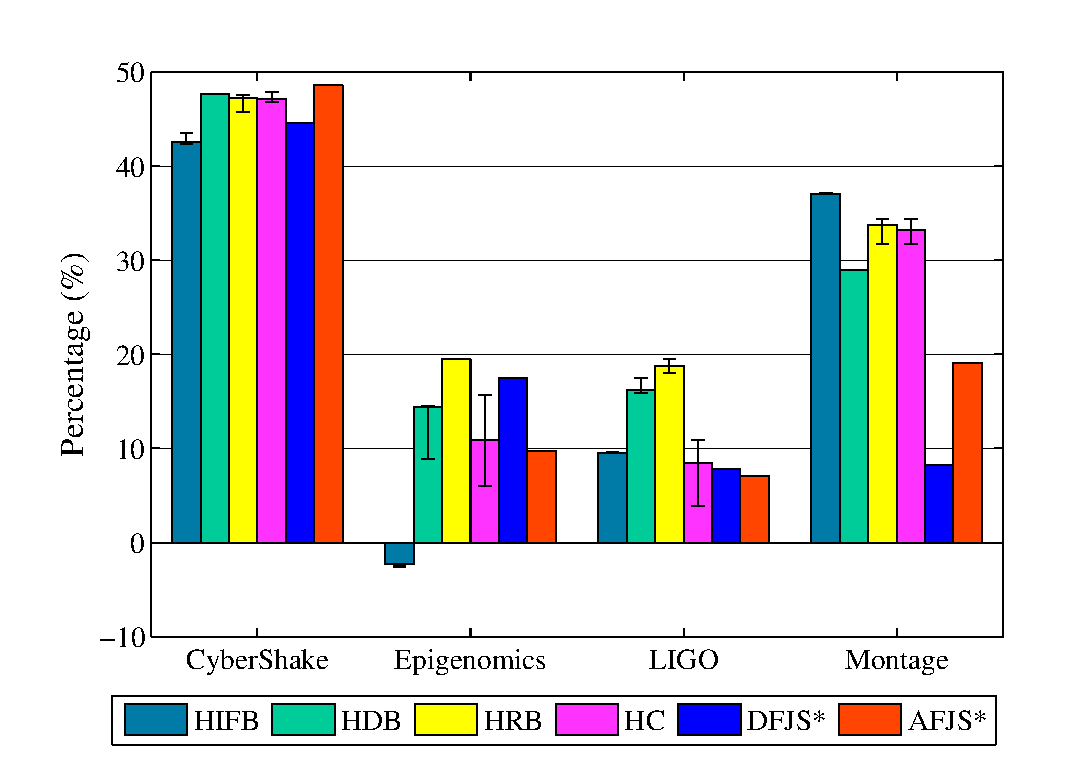
\includegraphics[width=1.0\linewidth]{figures/evaluation/algorithm2.eps}
	\captionof{figure}{Performance Gain over No Clustering of Six Algorithms (* indicates the best performance of DFJS and AFJS)}
	\label{fig:evaluation_algorithm}
\end{figure}

\begin{figure*}[!htb]
	\centering
    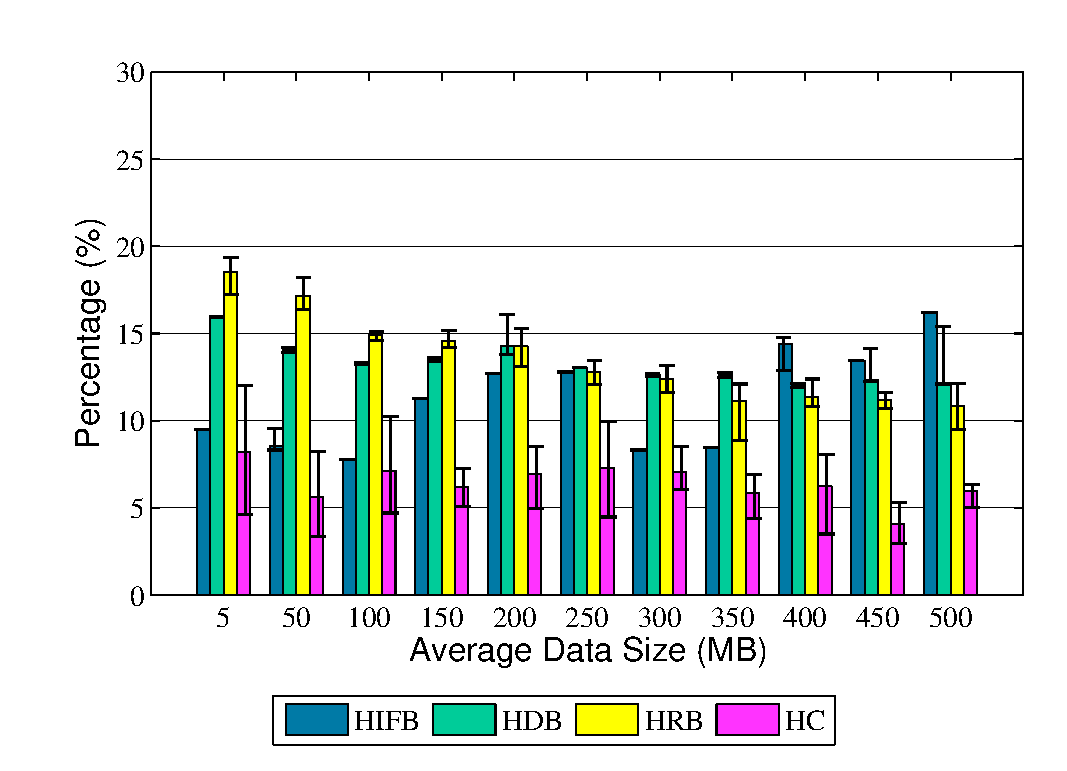
\includegraphics[width=0.7\textwidth]{figures/evaluation/datasize2.eps}
    \caption{Performance Gain over No Clustering with Different Data Size}
    \label{fig:evaluation_datasize}
\end{figure*}

\begin{figure}[!htb]
	\centering
	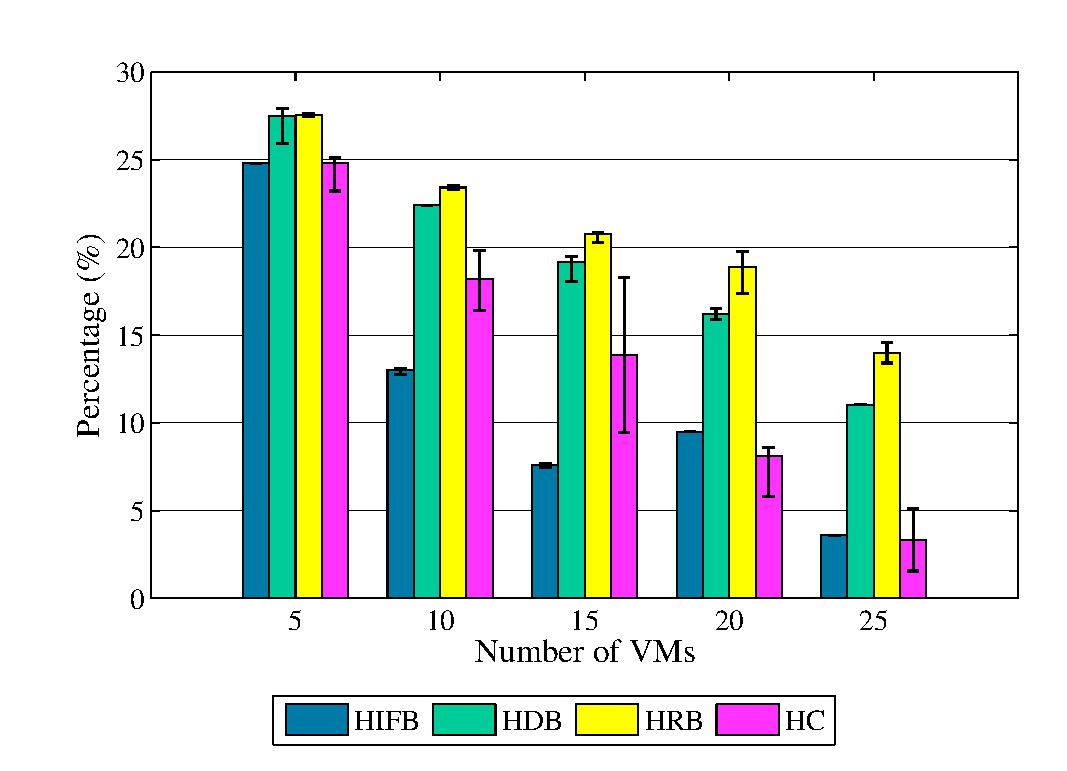
\includegraphics[width=1.0\linewidth]{figures/evaluation/resource1.eps}
	\captionof{figure}{Performance Gain over No Clustering with Different Number of Resources (Average data size is 5MB).}
	\label{fig:evaluation_resource_1}
\end{figure}

\begin{figure}[!htb]
	\centering
	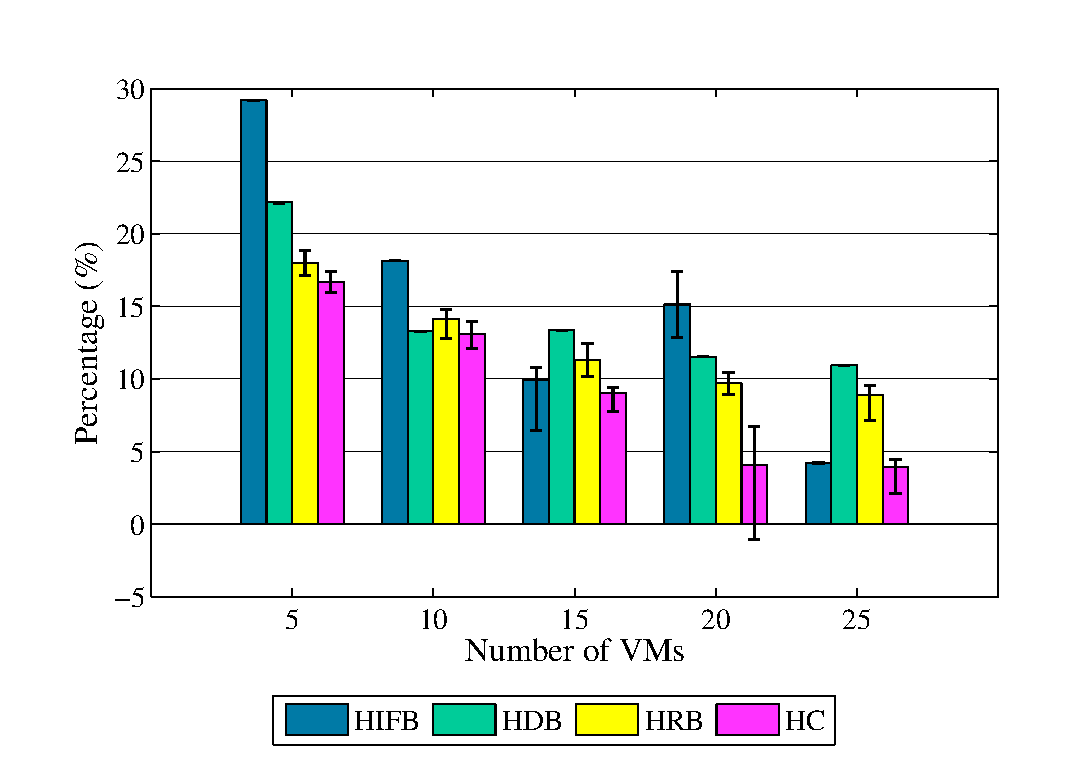
\includegraphics[width=1.0\linewidth]{figures/evaluation/resource2.eps}
	\captionof{figure}{Performance Gain over No Clustering with Different Number of Resources (Average data size is 500MB)).}
	\label{fig:evaluation_resource_2}
\end{figure}


Experiment 2: Fig.~\ref{fig:evaluation_datasize} shows the performance gain of HIFB, HDB, HRB and HC for the LIGO Inspiral workflow. The reason we chose the LIGO Inspiral workflow is that it has most significant difference among these methods. It is clear that with the increase of average data size, HIFB performs better and better while HRB performs worse. We don't see much difference of HC and HDB while varying data size. The reason is HIFB is able to capture the structural and runtime information, reducing data transfers between tasks, while HRB focuses on runtime distribution only. Therefore, while the workflow is more data intensive, we observe better performance of HIFB and a worse performance of HRB. HC does not change much since it is randomly merges tasks at the same horizontal level without information about runtime or data dependency. HDB does not change much since its performance gain is already good enough. 


\begin{figure}[!htb]
	\centering
	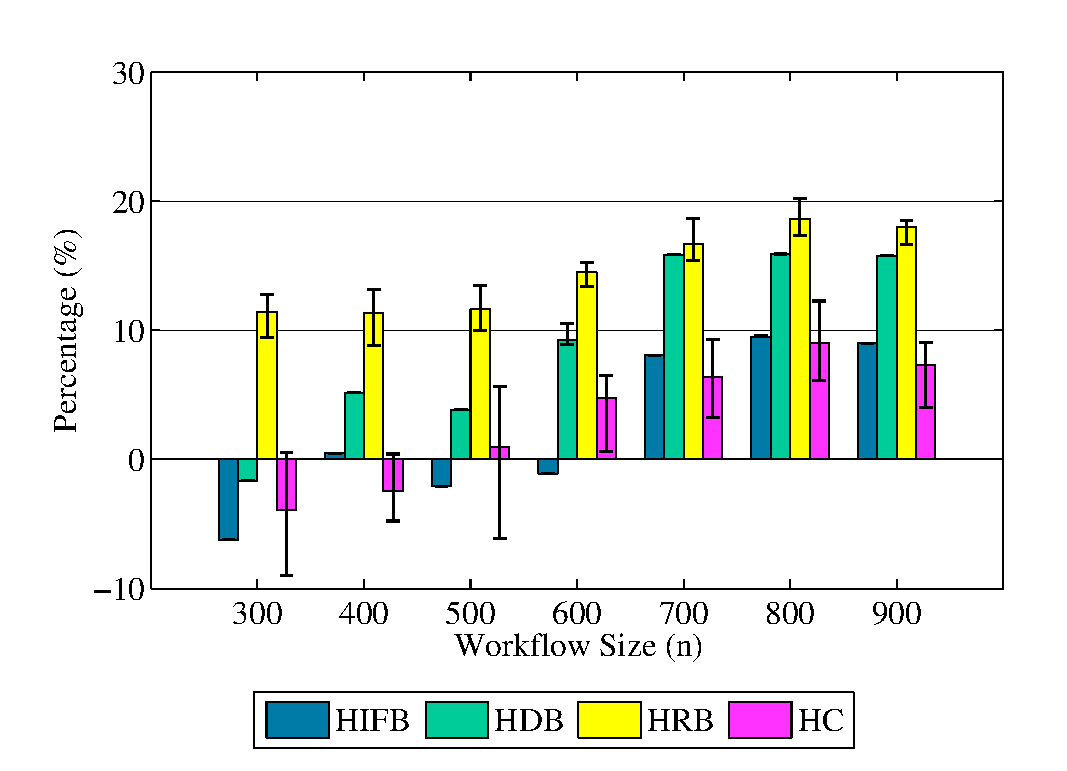
\includegraphics[width=1.0\linewidth]{figures/evaluation/workflowsize.eps}
	\captionof{figure}{Performance Gain over No Clustering with different Workflow Sizes}
	\label{fig:evaluation_wfsize}
\end{figure}

\begin{figure}[!htb]
	\centering
	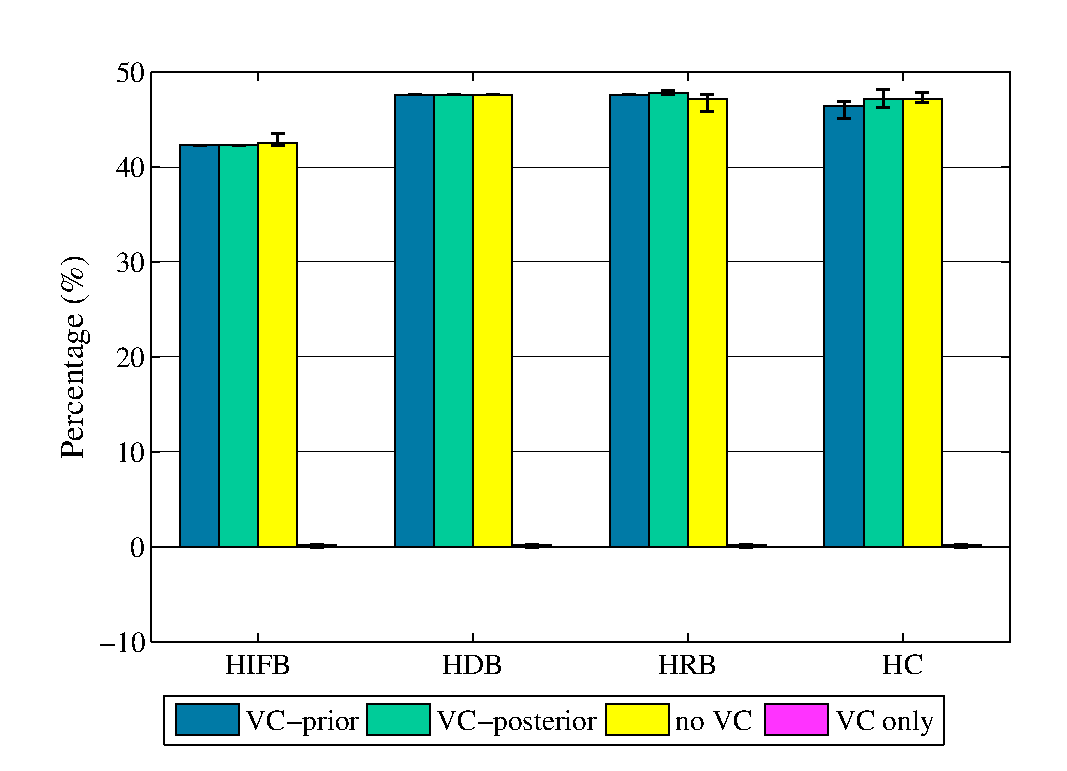
\includegraphics[width=1.0\linewidth]{figures/evaluation/vc_cybershake2.eps}
	\captionof{figure}{Performance Gain over No Clustering for Vertical Methods (CyberShake)}
	\label{fig:evaluation_vc_cybershake}
\end{figure}



\begin{figure}[!htb]
	\centering
    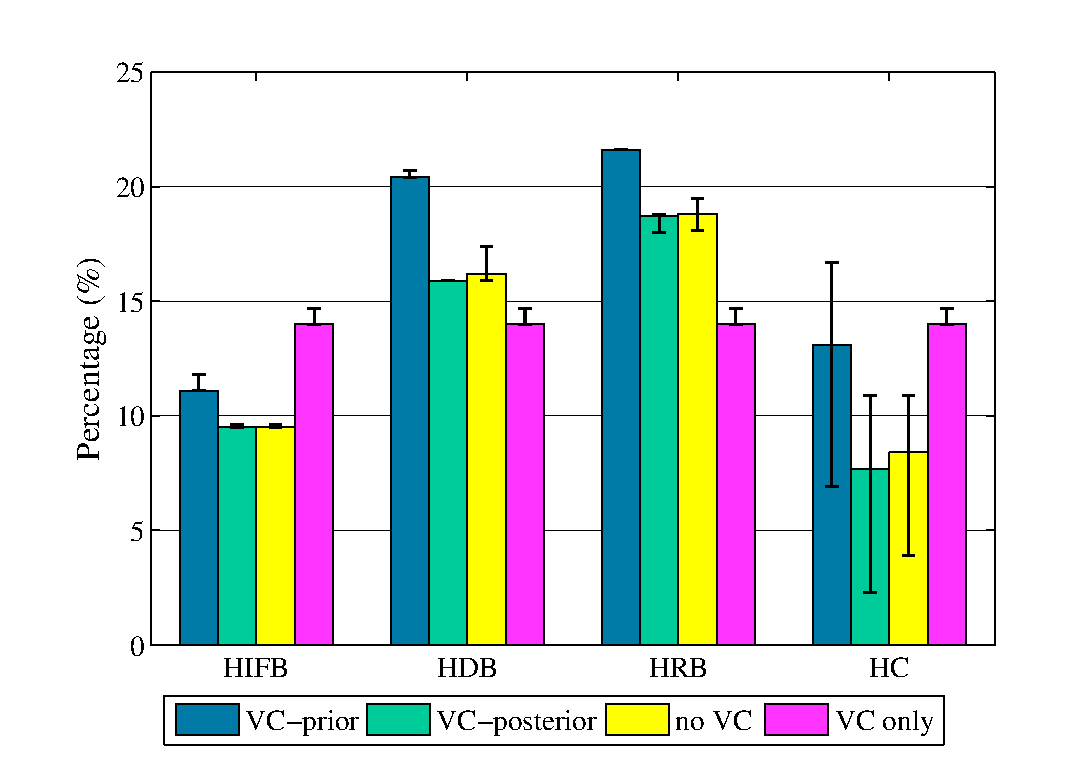
\includegraphics[width=1\linewidth]{figures/evaluation/vc_ligo2.eps}
    \captionof{figure}{Performance Gain over No Clustering for Vertical Methods (LIGO)}
    \label{fig:evaluation_vc_ligo}
\end{figure}


\begin{figure}[!htb]
	\centering
	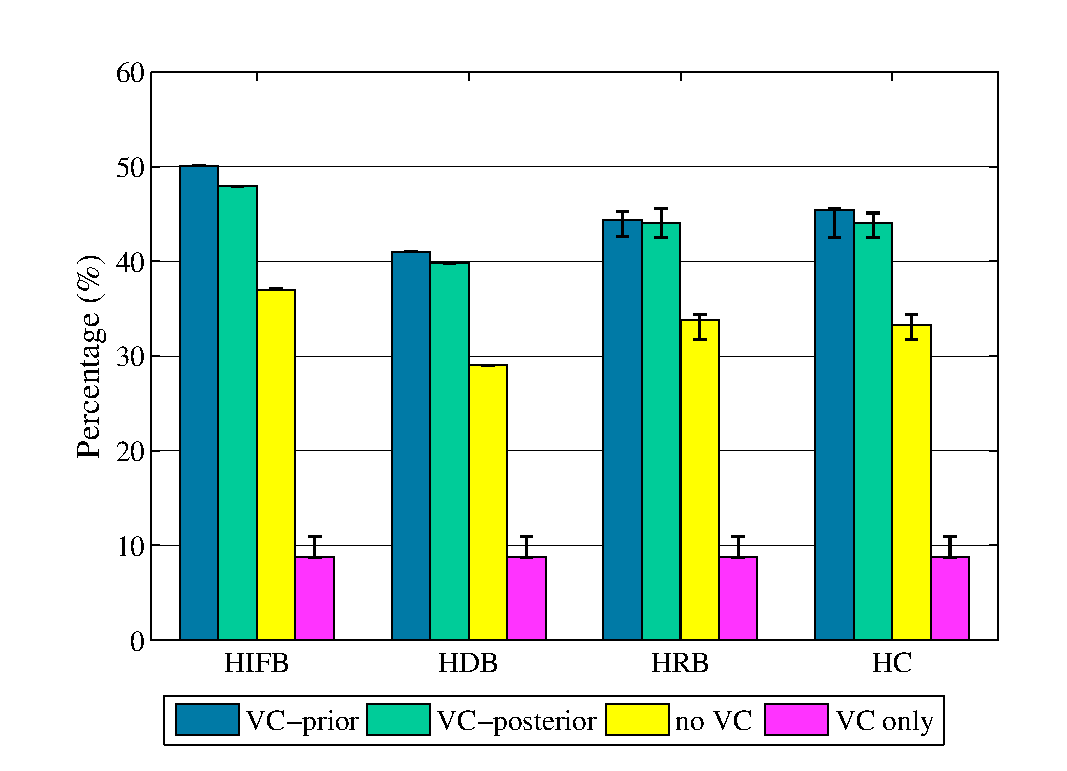
\includegraphics[width=1.0\linewidth]{figures/evaluation/vc_montage2.eps}
	\captionof{figure}{Performance Gain over No Clustering for Vertical Methods (Montage)}
	\label{fig:evaluation_vc_montage}
\end{figure}

\begin{figure}[!htb]
	\centering
	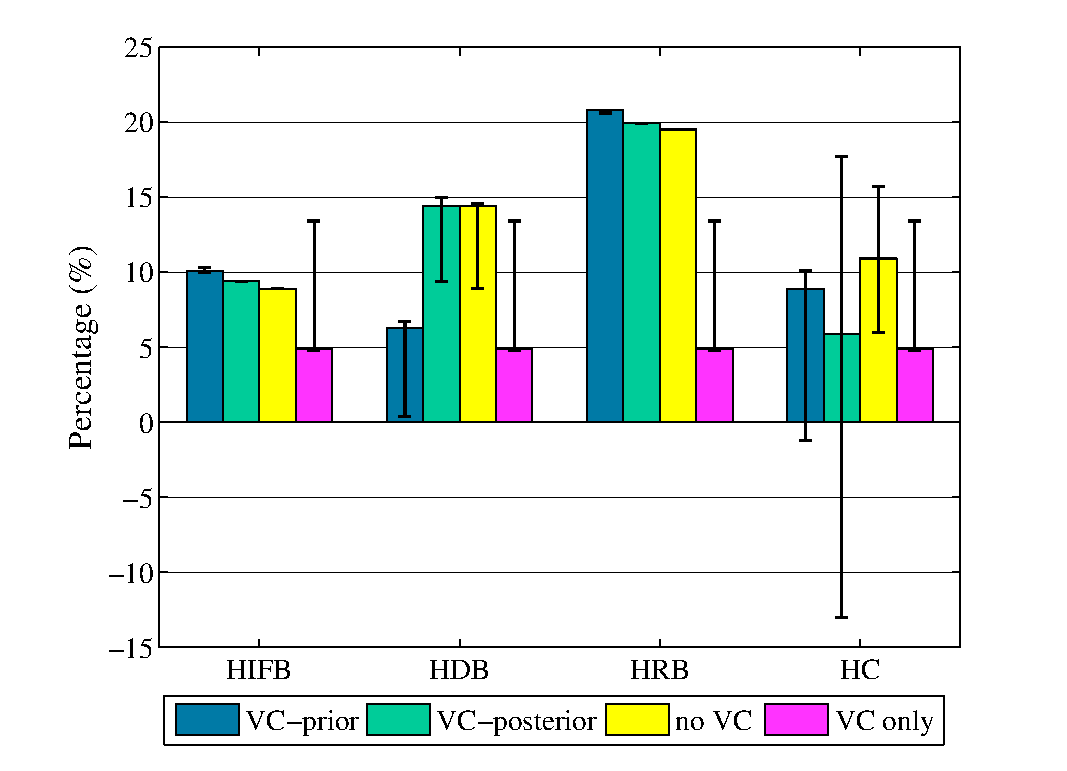
\includegraphics[width=1.0\linewidth]{figures/evaluation/vc_genome2.eps}
	\captionof{figure}{Performance Gain over No Clustering for Vertical Methods (Genome)}
	\label{fig:evaluation_vc_genome}
\end{figure}

\begin{table}[!htb]
\caption{Imbalance Metrics (Montage)}
\label{tab:evaluation_montage}
\centering
\begin{tabular}{lrrrrrrrr}
\hline
Level & Tasks & HRV &  HIFV & HDV  \\

\hline
1 &49 & 0.022 & 0.007 & 189.170 \\
2 & 196 & 0.010 & 0 & 0\\
3 & 1 & 0 & 0 & 0\\
4 & 1 & 0 & 0 & 0\\
5 &49 & 0.017 & 0 & 0\\
6 & 1 & 0 & 0 & 0 \\
7 &1  & 0 & 0 & 0\\
8 &1 & 0 & 0 & 0\\
9 & 1 & 0 & 0 & 0\\
\hline
\end{tabular}
\end{table} 

\begin{table}[!htb]
\caption{Imbalance Metrics (Epigenomics)}
\label{tab:evaluation_genome}
\centering
\begin{tabular}{lrrrrrrrr}
\hline
Level & Tasks & HRV &  HIFV & HDV  \\

\hline
1 & 3 & 0.327 & 0 & 0 \\
2 & 39 & 0.393 & 0 & 578\\
3 & 39 & 0.328 & 0 & 421\\
4 & 39 & 0.358 & 0 & 264\\
5 &39 & 0.290 & 0 & 107\\
6 & 3 & 0.247 & 0 & 0 \\
7 &1  & 0 & 0 & 0\\
8 &1 & 0 & 0 & 0\\
9 & 1 & 0 & 0 & 0\\
\hline
\end{tabular}
\end{table} 

\begin{table}[!htb]
\caption{Imbalance Metrics (CyberShake)}
\label{tab:evaluation_cybershake}
\centering
\begin{tabular}{lrrrrrrrr}
\hline
Level & Tasks & HRV &  HIFV & HDV  \\

\hline
1 & 4 & 0.309 & 0.031 & 1.225 \\
2 & 347 & 0.282 & 0 & 0\\
3 & 348 & 0.397 & 0 & 26.2\\
4 & 1 & 0 & 0 & 0 \\

\hline
\end{tabular}
\end{table} 


\begin{table}[!htb]
\caption{Imbalance Metrics (LIGO)}
\label{tab:evaluation_ligo}
\centering
\begin{tabular}{lrrrrrrrr}
\hline
Level & Tasks & HRV &  HIFV & HDV  \\

\hline
1 & 191 & 0.024 & 0.01 & 10097 \\
2 & 191 & 0.279 & 0.01 & 8264\\
3 & 18 & 0.054 & 0 & 174\\
4 & 191 & 0.066 & 0.01 & 5138\\
5 & 191 & 0.271 & 0.01 & 3306\\
6 & 18 &  0.04 & 0 & 43.7\\

\hline
\end{tabular}
\end{table} 


\begin{table}[!htb]
\caption{Imbalance Metrics (LIGO after performing VC)}
\label{tab:evaluation_ligo_vc}
\centering
\begin{tabular}{lrrrrrrrr}
\hline
Level & Tasks & HRV   \\

\hline
1,2 & 191 & 0.271  \\
3 & 18 & 0.054 \\
4,5 & 191 & 0.268 \\
6 & 18 &  0.04 \\

\hline
\end{tabular}
\end{table} 


Fig.~\ref{fig:evaluation_resource_1} and Fig.~\ref{fig:evaluation_resource_2} vary the number of VMs with an average data size of 5MB and 500MB respectively. We can see that with the increase of VMs, the performance gain of all of these methods decrease while HIFB and HDB decrease more significantly than HRB and HC. The reason is similar to the case of Fig.~\ref{fig:evaluation_datasize} since HIFB and HDB are data dependency aware. The difference between HDB and HIFB is HDB captures the strong connections between tasks (data dependencies) and HIFB captures the weak connections (similarity in terms of structure). In some cases, HIFV is zero (i.e, Epigenomics) while HDV is less unlikely to be zero. Fig.~\ref{fig:evaluation_wfsize} compares the performance gain of these algorithms by varying the workflow sizes (number of tasks in a workflow). By default, the LIGO Inspiral workflow in our paper has 800 tasks. With the decrease of workflow size, we can see that all of these methods perform worse. The reason is there is less resource contention with the decrease of workflow size and therefore task clustering does not perform well. The performance of HRB is more stable since the increase (or decrease) of workflow size has more significant impact on data transfer (roughly linear increase in runtime and square increase in data transfer). 

Experiment 3: Fig.~\ref{fig:evaluation_vc_cybershake},~\ref{fig:evaluation_vc_ligo},~\ref{fig:evaluation_vc_montage} and ~\ref{fig:evaluation_vc_genome} show the performance gain of combining VC along with our horizontal methods with four workflows respectively. For the CyberShake workflow as shown in Fig.~\ref{fig:evaluation_vc_cybershake}, we do not observe any significant change with VC since CyberShake does not have an explicit pipeline that we can perform vertical clustering (the performance gain of VC only is almost zero). 


For the LIGO Inspiral workflow as shown in Fig.~\ref{fig:evaluation_vc_ligo}, we can see that VC-prior perform better than other combination approaches. The reason is VC-prior increases HRV and allows horizontal methods to improve the performance further while VC-posterior does not have many tasks to merge since horizontal methods change the pipeline structures. Table.~\ref{tab:evaluation_ligo_vc} shows the HRV after we perform VC on the LIGO Inspiral workflow. 

For the Montage workflow as shown in Fig.~\ref{fig:evaluation_vc_montage}, we do see significant improvement with VC (about 15\% more than the case without VC). However, the performance improvement does not distinguish these horizontal methods. The reason is tasks merges by VC (the middle and the tail levels of Montage as shown in Fig.\ref{fig:evaluation_shape_montage})are different from the one merged by horizontal methods (the first two levels in Fig.~\ref{fig:evaluation_shape_montage}). Therefore, the performance of VC-posterior and VC-prior does not differ from each other.  


For the Epigenomics workflow as shown in Fig.~\ref{fig:evaluation_vc_genome}, we observe similar phenomenon in HRB compared to the LIGO Inspiral workflow. As to the performance of HDB, VC-prior merges tasks at the second, third, fourth and fifth level together and thus HDB has less space to further improve the overall runtime. 
 
%HIFB and HDB significantly increase the performance of the workflow execution. Both strategies capture the structural and runtime information, reducing data transfers between tasks, while HRB focuses on runtime distribution, which in this case is none. Fig.~\ref{fig:imbalance_performance} (bottom) shows the performance of the balancing methods for the Epigenomics workflow. When increasing the average data size, only HDB demonstrates significantly improvement related to HC. Investigating the structure of the Epigenomics workflow (Fig.~\ref{fig:imbalance_shape}-bottom), we can see that all tasks at the same horizontal level share the same IFs ($HIFV$ = 0), because each branch (surrounded by dash lines) happen to have the same amount of pipelines. Thus, HIFB has no performance improvement when compared to HC. However, for LIGO (Fig.~\ref{fig:imbalance_shape}-top), $HIFV \neq 0$, thus HIFB improves the workflow runtime performance.  
%The intuition behind this difference between HDB and HIFB is that 
%HDB captures the strong connections between tasks (data dependencies) and HIFB captures the weak connections (similarity in terms of structure). In both workflows, $HDV$ is not zero thus HDB performs better than HC. 







\section{Conclusion and Future Work}

We presented three balancing methods and two vertical clustering combination approaches to address the load balance problem when clustering workflow tasks. We defined three imbalance metrics to quantitatively measure workflow characteristics based on task runtime variation (HRV), task impact factor (HIFV), and task distance variance (HDV).

Three experiment sets were conducted using five real workflow traces. The first experiment showed the performance gain over a control execution that has no clustering. Our clustering techniques are comparable (and in some cases much better than) to three existing algorithms. The second experiment showed the influence of average data size and number of VMs on the performance gain. Particularly, it showed that the three clustering algorithms have different sensitivity to data intensive workflows and computation intensive workflows. The last experiment showed the performance gain of combining 

In the future, we are going to further analyze the imbalance metrics proposed. For example, the values of these metrics presented in this paper are not normalized and thus their values per level (HIFV, HDV and HRV) are in different scales. Also, we are going to analyze more workflow examples, particularly the ones with asymmetric workflow structures, to illustrate the relationship between workflow structures and the metric values. 

As shown in this paper, the three balancing algorithms and the two vertical clustering combination approaches have different sensitivity to workflows with different graph structures and runtime distribution. Another future work is portfolio scheduling, which chooses multiple scheduling algorithms initially and selects dynamically a suitable algorithm from them according to the dynamic load. 

\section{Acknowledgements}
This work is funded by NSF IIS-0905032 and NSF FutureGrid 0910812. We thank Gideon Juve, Karan Vahi, Rajiv Mayani and Mats Rynge for their help. 





%% References with bibTeX database:

\bibliographystyle{elsarticle-num}
\bibliography{biblio}

\end{document}